\documentclass[logo,civil,dosguias]{tesis-pregrado}
% opciones: logo,dosguias,civil,ejecucion,propuesta,txfonts

\keywords{Memetic Algorithm; Protein Structure Prediction}

\begin{document}
\baselineskip 25pt
% ----------------------------------------------------------
% ----------- PARTE INICIAL --------------------------------
\thispagestyle{empty}
% Rellenar con la informacion personal y del trabajo

\titulo{Algoritmo mem\'etico para el problema de predicci\'on de la estructura tridimensional de una prote\'ina}

\autor{Camilo Javier Farf\'an P\'erez}
\email{camilo@requies.cl}
\telefono{+569 8640 1812}
\run{17.150.968-8}
\annoingreso{2008}

\fecha{Martes}{21}{Abril}{2015}

\profesorguia{Mario Inostroza Ponta, PhD}
\profesorcoguia{Dr.\ Marcio Dorn}

\ciudad{Santiago}
\pais{Chile}

\makecubierta

\makecopyright % si es propuesta no se mostrará
% ----------------------------------------------------------
% ----------- PRIMERA PARTE --------------------------------
\frontmatter
% ### Resumen e Indices ####
%
\begin{gracias}

\end{gracias}
%
\dedicatoria{
  Dedicado a mi familia, en especial a mi mamá Ivonne.
}


\resumenCastellano{
El entendimiento de los procesos biológicos ha sido un desafío permanente para la humanidad. Debido a la gran cantidad de información biológica que se dispone, es que nace la bioinformática, área que se encarga de apoyar a la biología con técnicas computacionales para el tratamiento y análisis de información. Dentro de los desafíos que expone, se encuentra el problema de predicción de la estructura tridimensional de la proteína (3-D PSP), este problema es del tipo NP-Completo. Los intentos por resolverlo han implicado la construcción de las más potentes supercomputadoras solo para entender cómo funciona el proceso de plegamiento, en el cual las moléculas usando la menor cantidad de energía se disponen espacialmente en un medio acuoso. Debido al costo computacional de este problema, es que existen diversas técnicas heurísticas que sacrifican precisión por tiempo de ejecución pero que se presentan como herramientas computacionalmente viables.

En este trabajo se presenta un algorítmo memético que usa información experimental extraída de la \textit{Protein Data Bank} para resolver el problema de la predicción de la estructura terciaria de la proteína. La información extraída está dispuesta como una Lista de Probabilidad de Ángulos (APL), su principal función es descartar aquellos valores que no presentan relevancia biológica al poseer una ocurrencia nula o de muy baja probabilidad. Este algoritmo hace uso de técnicas que han demostrado ser útiles en otras áreas. En específico, se usa una adaptación del método de recocido simulado como estrategia de búsqueda y una estructura jerárquica de población compuesta por 13 agentes. 

La etapa de pruebas contempla comprobar la contribución de la APL, para ello se realizó 20 ejecuciones por cada una de las seis proteínas en estudio. Las 20 ejecuciones se dividen en 10 ejecuciones que incorporan la información de APL, y 10 que usan valores aleatorios. Los resultados obtenidos son satisfactorios y cumplen los objetivos planteados en este trabajo. Se logra demostrar la contribución de la APL, reflejado en el análisis de superposición de estructuras, obteniéndose RMSDs menores a 1$\AA$. Las predicciones realizadas logran simular correctamente las hojas hélices de las estructuras, no asi las hojas-$\beta$. El comportamiento del MA en proteínas de mayor longitud se mantiene al arrojar resultados con RMSDs bajos. 

Finalmente, los resultados obtenidos fueron aceptados para su exposición en la \textit{Genetic and Evolutionary Computation Conference} (GECCO 2015) a efectuarse en Madrid, España los días 11 al 15 de Julio de 2015.
\vspace*{0.5cm}
\KeywordsES{Algoritmos meméticos; Bioinformática Estructural; Predicción de la estructura tridimensional de la proteína}
}

%\newpage

%\resumenIngles{

%\vspace*{0.5cm}
%\KeywordsEN{Memetic Algorithms; Protein Structure Prediction; Structural Bioinformatics}
%}

\pagestyle{fancy}
\fancyhead[L]{\slshape \leftmark}
\fancyhead[C]{}
\fancyhead[R]{\thepage}
\tableofcontents        %% Indice general
\listoffigures          %% Indice de figuras
\listoftables           %% Indice de tablas
\listofalgorithms       %% Indice de algoritmos
% ----------------------------------------------------------
% ----------- SEGUNDA PARTE --------------------------------
\mainmatter
% ### Configuración del header ###
\pagestyle{fancy}
\fancyhead[L]{\slshape \leftmark}
\fancyhead[C]{}
\fancyhead[R]{\thepage}
\pagenumbering{arabic}
% ### Capitulos de la tesis ###
\baselineskip 25pt
\chapter{Introducci\'on}
\label{cap:intro}
En este capítulo el lector encontrará los elementos y conceptos introductorios necesarios para el entendimiento de este trabajo de título. 

\section{Antecedentes y motivaci\'on}
\label{intro:motivacion}

Con el paso del tiempo la tecnología avanza de forma considerable, lo que ha permitido el desarrollo de distintas áreas de la ciencia. Una de ellas es la Biología, área capaz de generar grandes volúmenes de información. Todo este conjunto de datos debe ser evaluado y estudiado, es así como nace la Bioinformática, campo de la Informática centrada en apoyar a la biología mediante el análisis y procesamiento de información biológica (\citealp{bioinf:def}).

Dentro de la Bioinformática, se encuentra la Bioinformática Estructural que se encarga principalmente del análisis y predicción de las estructuras tridimensionales de macro-moléculas biológicas (\citealp{bioinf:struct}), como el ADN, ARN y proteínas. El problema de la predicción de la estructura tridimensional de la proteína se conoce por sus siglas en inglés como \textit{3-D PSP (Three-dimensional Protein Structure Prediction) Problem} y es en el cual se basa este trabajo.

La estructura 3-D de la proteína da importante información acerca de su función biológica. Por ejemplo, la hemoglobina es la proteína encargada de transportar oxígeno en la sangre, para ello debe poseer una estructura tridimensional adecuada para poder realizar dicha tarea, para ello debe poseer zonas de anclaje que permitan a la hemoglobina captar moléculas de oxígeno. Por lo tanto, si se logra simular la estructura de tridimensional con una precisión alta implicaría un paso importante en el diseño de proteínas con fines específicos, lo anterior corresponde a la base del desarrollo de fármacos y drogas (\citealp{Cohen19961}).

No obstante, a pesar de los avances científicos, este problema sigue siendo costoso computacionalmente debido a la gran cantidad de recursos que se necesita para la simulación de interacciones moleculares. Además estas simulaciones se efectúan bajo la siguiente restricción biológica: la formación de la estructura tridimensional de la proteína se debe realizar usando la menor energía posible (\citealp{Anfinsen:1972}). Esto implica que cada modificación a nivel estructural tendrá repercución en la energía potencial libre del sistema, lo que complica y encarece el problema a nivel computacional.

Según lo revisado en \citealp{Zhang:2008}, se considera que los resultados cuyo RMSD entre $3-5\AA$ poseen una correcta topología, no asi aquellas que obtienen RMSD mayor a $9\AA$, de las cuales se dice que su topología es incorrecta. Además, menciona algunas técnicas que logran buenos resultados como ROSSETA (\citealp{Simons1997209}, con un promedio RMSD de $1.8\AA$ para la proteína CASP T0283 con 92 residuos de aminoácidos y un tiempo de 150 días de cómputo. I-TASSER (\citealp{PROT:PROT21702}) con resultados entre los $3-9\AA$ para proteínas de hasta 155 residuos y ASTRO-FOLD (\citealp{PROT:PROT20338}) con $5.2\AA$ para proteínas de 102 residuos.

\section{Descripci\'on del problema}
\label{intro:problema}

El problema de predicción de la estructura tridimensional de la proteína se resume en, encontrar la conformación tridimensional de la secuencia de aminoácidos con el mínimo de energía posible (\citealp{Anfinsen:1972}). Este problema pertenece al grupo NP-Completo (\citealp{Crescenzi:1998}) y se enmarca como uno de los principales desafíos en el área de la bioinformática estructural.

Las proteínas están compuestas por áminoácidos unidos mediantes enlaces. En estos enlaces se encuentran los ángulos de torsión o ángulos diedros que le dan la forma tridimensional a la proteína. El proceso de plegado ocurre de tal forma que la energía usada en este evento sea la mínima. Como se puede inferir, a medida que se aumenta la cantidad de residuos aumenta el espacio de soluciones debido a la cantidad de combinaciones posibles (\citealp{Zhang:2008}).

Los enlaces entre aminoácidos se conocen como enlaces peptídicos. Estos son producto de la interacción entre el grupo carboxilo y amino de los residuos. La principal particularidad que presentan las zonas enlazadas es la flexibilidad, que da origen a ángulos que terminan por dar forma al péptido. Estos ángulos son conocidos como diedros o de torsión, representados por las letras griegas $\phi$ y $\psi$ (\citealp{molecular:book}). Estos ángulos pueden tomar valores entre los $-180^{\circ}$ y $180^{\circ}$, es decir, para el par ($\phi$,$\psi$) existen $360{\times}360$ posibilidades, si la precisión de los ángulos se extiende a 3 decimales las posibilidades aumentan a $12.96{\times}10^{10}$. Por lo tanto, a medida que la proteína posee más residuos o aminoácidos, la cantidad de posibles conformaciones tridimensionales aumenta considerablemente lo que, en consecuencia, significa un espacio de búsqueda intratable. Desde el punto de vista de la dinámica molecular, es posible simular el proceso de plegado. No obstante, realizar esta simulación también es complicada y costosa computacionalmente hablando, debido a la gran cantidad de átomos, interacciones y variables termodinámicas involucradas. 

Para resolver este problema se han propuesto diversos enfoques, metodologías, sistemas y algoritmos que pueden ser agrupados en 4 clases:
\begin{itemize}
    \item Métodos \textit{ab initio} sin información de bases de datos.
    \item Métodos \textit{ab initio} con información de bases de datos.
    \item Métodos de enhebrado y reconocimiento de plegamientos.
    \item Métodos de modelamiento por comparación y estrategias de alineamiento de secuencias.
\end{itemize}
La primera clase corresponde a técnicas cuya principal ventaja es predecir estructuras nuevas o \textit{de novo} a través de la simulación de las propiedades físicoquímicas del proceso de plegamiento de la proteína. Las demás clases corresponden a métodos mucho más rápidos y efectivos para la predicción de estructuras tridimensionales, ya que hacen uso de plantillas estructurales y de bibliotecas de estructuras conformacionales conocidas (\citealp{Dorn2014251}). Estos enfoques serán explicados en detalle en la sección \ref{fundamentos:estado-arte} correspondiente al estado del arte.


\subsection{Enunciado del problema}
\label{intro:enunciado}
Dada una secuencia de aminoácidos se debe predecir la estructura tridimensional (estructura terciaria) de la proteína que representa.

\section{Soluci\'on propuesta}
\label{intro:solucion}

\subsection{Prop\'osito de la solución}

El propósito de la solución es, generar predicciones de proteínas a nivel de estructura terciaria usando los ángulos obtenidos de bases de datos experimentales. La idea de usar estos ángulos es disminuir el espacio de búsqueda, ya que se dejan de visitar aquellas regiones que los datos experimentales demuestran no tener relevancia. En la figura \ref{fig:rmc-proline} se puede apreciar que hay 2 zonas en las que se concentran los ángulos usados por el aminoácido \textit{Prolina}. Esto demuestra que no tiene sentido incluir en las simulaciones aquellas regiones que el aminoácido experimentalmente no usa. 

\begin{figure}[tp]
	\centering
	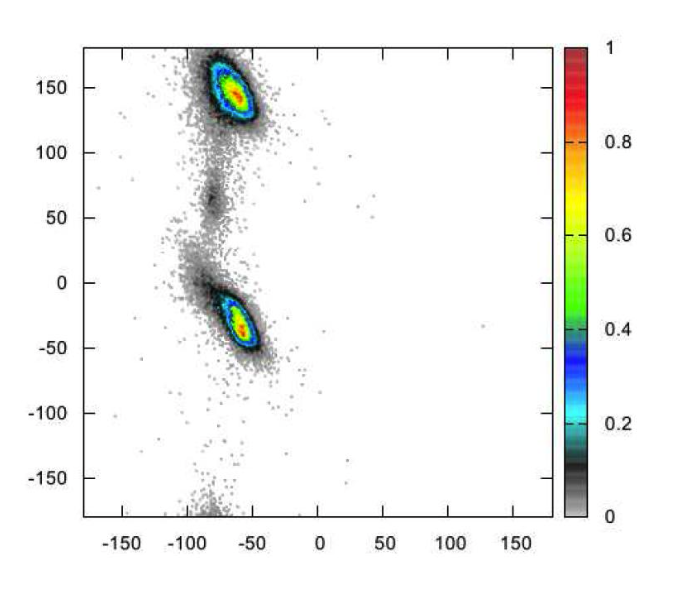
\includegraphics[scale=.35]{images/rmc-proline.png}
	\caption{\em Mapa de Ramachandran para las ocurrencias de los ángulos $\phi$ y $\psi$ encontrados en la Protein Data Bank para el amino\'acido Prolina (\citealp{Dorn:2013}).}
	\label{fig:rmc-proline} 
\end{figure}

Para llevar a cabo el propósito, se ha desarrollado un algoritmo memético que incorpora la información de los ángulos diedros más probables. Su objetivo es tomar y generar modelos candidatos de estructuras bajo la aplicación de operadores propios de los algoritmos evolutivos, que son mejorados mediante un operador de búsqueda local. El enfoque de esta solución está enmarcada dentro de las técnicas \textit{ab initio} que usan información de bases de datos cuya descripción detallada se encuentra en la sección \ref{fundamentos:abinitio-db}.

Los datos a emplear son provistos por la \textit{Protein Data Bank} (\citealp{Berman:2000}), que cuenta con la información de los ángulos de torsión $\phi$ y $\psi$ de estructuras conocidas y comprobadas experimentalmente a través de métodos de Cristalografía de Rayos X o Resonancia Magnética Nuclear (\textit{Nuclear Magnetic Resonance, NMR}). Para más detalle de estos métodos experimentales, revisar sección \ref{fundamentos:estructura-terciaria}.

\subsection{Alcances y limitaciones de la solución}

La solución enmarca las siguientes aristas y limitantes:

\begin{enumerate}[a)]
\item La solución propuesta contempla la evaluación e implementación solo para estructuras terciarias de proteínas y está basada en la solución propuesta en \cite{Dorn:2013}.
\item Solo se usan proteínas de acceso público disponibles en la \textit{Protein Data Bank} con solo una cadena principal de aminácidos.

\item Para el estudio y evaluación solo se consideran las proteínas 1DEP, 1E0Q, 1K43, 1L2Y, 1RPV y 2EVQ, cualquier otra proteína mencionada o evaluada en este trabajo es con fines ilustrativos.

\item No se considera una solución a nivel distribuido, por lo que la solución solo hace uso de los recursos provistos por el dispositivo de ejecución.
\end{enumerate}


\section{Objetivos}
\label{intro:objetivos}

En esta sección se dan a conocer los objetivos del presente trabajo, tanto en su enfoque general como en sus puntos específicos.

\subsection{Objetivo general}

El objetivo general de este trabajo es: la implementación de un algoritmo memético que incorpore conocimiento biológico y permita encontrar soluciones de buena calidad biológica para el problema \textit{3-D PSP}.

\subsection{Objetivos espec\'ificos}

Para la consecución del objetivo general, se plantean las siguientes metas intermedias:

\begin{enumerate}
  \item Reducción del espacio de búsqueda conformacional de la proteína, mediante el uso de una lista de probabilidades de ocurrencia (\textit{Angle Probability List, APL}) de pares de ángulos $\phi$ y $\psi$.
  \item Diseño e implementación del algoritmo memético que use la información biológica entregada por la APL.
  \item Diseño e implementación de un operador de búsqueda local para el algoritmo memético.
  \item Comparación y análsis de resultados con datos experimentales.
\end{enumerate}

\section{Metodolog\'ia y herramientas utilizadas}
\label{intro:metodologia}

\subsection{Metodolog\'ia}

Por tratarse de un tema de investigación y experimentación, se usará el método científico como metodología de foco para el desarrollo de este trabajo de título.

La hipótesis del trabajo es: \textbf{``Incorporar las probabilidades de ángulos de torsión $\phi$ y $\psi$ en un algoritmo memético permite obtener predicciones de estructuras tridimensionales de proteína de mejor calidad biológica''.}

No obstante, para realizar la etapa de experimentación para refutar o confirmar la hipótesis, es necesario la construcción de software, por lo que la metodología estará marcada por 4 etapas que se indican a continuación:

\begin{enumerate}
	\item \textbf{Concepción:} Se establecen los estudios necesarios para abordar el problema revisando alternativas y estrategias de solución.
	\item \textbf{Elaboración:} En esta etapa se definen modelos, esquemas y diagramas que se utilizan para construir la solución en base a la información recopilada en la concepción
	\item \textbf{Construcción:} Durante la construcción se implementan todos los elementos definidos durante la elaboración.
	\item \textbf{Experimentos computacionales y análsis de resultados:}: esta etapa recoge los resultados obtenidos a partir de la construcción para refinar y estabilizar el software. Se evalúa la hipótesis de acuerdo a los resultados obtenidos.
\end{enumerate}

\subsection{Herramientas de desarrollo}

A continuación se presentan las herramientas tanto de software como hardware que se utilizaron en este trabajo de título.

\subsubsection{Herramientas de software}
Para la escritura del documento se usaron las siguientes herramientas:
\begin{itemize}
	\item Sistema Operativo OS X Yosemite versión 10.10
	\item LaTeX para Mac, MacTex versión 2014
	\item TexStudio versión 2.8.8
\end{itemize}

Para el desarrollo, compilación y ejecución de las implementaciones se utilizó:

\begin{itemize}
	\item Sistema Operativo Linux Ubuntu Desktop versión 14.04.1 LTS
	\item Sublime Text versión 2.0.2
	\item AmberTools versión 14.23 (\citealp{amber14}).
	\item Stride (\citealp{Heinig01072004}).
	\item PyMol versión 1.6 (\citealp{pymol}).
	\item Procheck versión 3.5.4 (\citealp{procheck}).
	\item Profit versión 3.1 (\citealp{profit}).
\end{itemize}

\subsubsection{Herramientas de hardware}
Las ejecuciones de la implementación se llevaron a cabo en 10 computadores de escritorio modelo HP EliteDesk 800 G1-SFF con las siguientes características:

\begin{itemize}
	\item CPU Intel 3.4Ghz de 8 núcleos físicos.
	\item 8Gb de RAM (dos módulos de 8Gb de 1600Mhz).
\end{itemize}

\section{Organizaci\'on del documento}
\label{intro:organizacion}

El presente trabajo se compone por los siguientes capítulos:

\begin{itemize}
	%\item \textbf{Introducción: }este capítulo tiene la misión de introducir al lector en el contexto de este documento, abarcar los conceptos básicos para su entendimiento, enunciar el problema y solución propuesta, además de, mencionar la metodología y herramientas que usadas a lo largo del trabajo de titulación.
	\item \textbf{Capítulo 2. Fundamentos teóricos: }Para el entendimiento del problema es necesario definir y profundizar conceptos claves, que son usados en capítulos posteriores. Además se presenta el estado del arte de esta área.
	\item \textbf{Capítulo 3. Diseño e implementación de la solución: }este capítulo aborda el diseño de la solución propuesta en este trabajo. Por lo tanto, se menciona todo lo relacionado al algoritmo memético implementado, como la representación de las soluciones y el diseño algorítmico de los operadores.
	\item \textbf{Capítulo 4. Criterios de evaluación y experimentos: } Capítulo encargado de exponer la estrategia de evaluación y experimentación. En consecuencia, abarca el diseño de experimentos, carácterísticas y evaluación de las soluciones.
	\item \textbf{Capítulo 5. Resultados: }Los resultados de este trabajo están divididos en dos sub-secciones, la primera expone la calidad algorítmica de la implementación, tanto en la convergencia del algorítmo memético como en los parámetros que fueron usados en la etapa de experimentación.
La segunda evalúa los resultados a nivel biológico, se usan métricas que permiten evaluar la calidad biológica de los resultados obtenidos.
	\item \textbf{Capítulo 6. Conclusiones: }Finalmente se exponen las conclusiones obtenidas en este trabajo y se indican las posibles mejoras que puede tener para ser implementadas en un futuro.
\end{itemize}
\chapter{Fundamentos te\'oricos}
\label{cap:fundamentos}

En este capítulo se expone los conceptos importantes sobre el problema de predicción de la estructura tridimensional de la proteína (\textit{3-D PSP}) y su  estado del arte. 

\section{Problema de predicción de la estructura tridimensional de la proteína}

Este problema consiste en la predicción de las estructuras secundarias, terciarias y cuaternarias a partir de la estructura primaria (\citealp{Anfinsen:1973}).La estructura tridimensional de la proteína da importante información acerca de la función biológica de la proteína, ya que según su conformación estructural será su interacción con otras proteínas y moléculas. Es por ello que la solución a este problema se considera altamente importante para el área de desarrollo de fármacos y drogas, y para la biotecnología en el desarrollo de nuevas enzimas (\citealp{Cohen19961}).

\subsection{Estructura de la proteína}

Las proteínas son largas secuencias compuestas por 20 diferentes tipos de aminoácidos o residuos (ver tabla \ref{table:aminoacids}) unidos por enlaces peptídicos. Estos enlaces son la consecuencia de la unión de un grupo carboxilo de un aminoácido con el grupo amino de otro, produciéndose la liberación de una molécula de agua. Cada vez que se realiza un enlace peptídico la cadena comienza a crecer y a tomar forma debido a las fuerzas atómicas inherentes a este evento (\citealp{Anfinsen:1972}). En consecuencia, las estructuras comienzan a plegarse debido a las variaciones que se producen en los puntos de torsión de la proteína. Los ángulos en estos puntos se conocen como ángulos de torsión, y se les denomina con las letras griegas $\phi$ y $\psi$ a aquellos ángulos producidos por la unión de un átomo de Nitrógeno(\textit{N}) con un átomo de Carbono(\textit{C}), y un Carbono-alfa($C_{\alpha}$) con un Carbono(\textit{C}) respectivamente (\citealp{Anfinsen:1973}), tal como se puede apreciar en la figura \ref{fig:phi-psi-exam}.

\begin{table}[tp]
	\centering
	\caption[Listado de aminoácidos y sus códigos]{Listado de códigos de los 20 aminoácidos usados en el problema PSP}
	\begin{tabular}{|r|r|r|}
		\hline
		\textbf{Nombre residuo} & \textbf{Código 1 letra} & \textbf{Código 3 letras} \\ \hline
		Glicina 	        & G	& GLY	\\		
		Alanina 	        & A	& ALA	\\ 		
		Valina 	            & V	& VAL	\\  	
		Leucina 	        & L	& LEU	\\ 		
		Isoleucina 	        & I	& ILE	\\ 		
		Fenilalanina 		& F	& PHE	\\		
		Tirosina 			& Y	& TYR	\\	
		Triptófano 			& W	& TRP	\\
		Serina 	    		& S	& SER	\\	
		Treonina 			& T	& THR	\\	
		Cisteína 			& C	& CYS	\\
		Metionina 			& M	& MET	\\
		Ácido Aspártico     & D & ASP   \\
		Ácido Glutámico 	& E	& GLU	\\
		Histidina 			& H	& HIS	\\
		Lisina   			& K	& LYS	\\
		Arginina 			& R	& ARG	\\
		Asparginina 		& N	& ASN	\\
		Glutamina 			& Q	& GLN	\\
		Prolina 			& P	& PRO	\\ \hline
	\end{tabular}
	\label{table:aminoacids}
\end{table}

\begin{figure}[h]
	\centering
	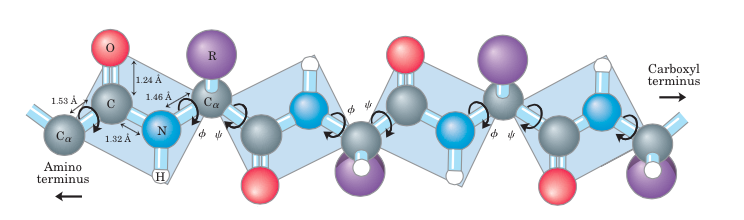
\includegraphics[scale=.6]{images/phipsi.png}
	\caption{\em \'Angulos de torsi\'on $\phi$ y $\psi$ (pág. 116 \citealp{lehninger}).}
	\label{fig:phi-psi-exam}
\end{figure}

Los cambios conformacionales de esta cadena son posibles debido a la rotación que ocurre en cada Carbono-\textalpha~($C_{\alpha}$). Además, cada aminoácido de la secuencia está polarizado, en otras palabras, tiene regiones positivas y negativas con un grupo \textit{C=O} libre, el cual puede actuar como receptor de un enlace de hidrógeno y un grupo \textit{NH} como donante de un enlace de hidrógeno.

Los 20 aminoácidos pueden ser clasificados de acuerdo a sus características químicas de la cadena lateral, que también juega un rol fundamental en la estructura 3-D. La Glicina, por ejemplo, tiene su cadena lateral más pequeña con solo un átomo de hidrógeno, lo que incrementa la flexibilidad de la estructura de la proteína (\citealp{Uzman:2001}). Por otro lado, la Cistina puede reaccionar con otra Cistina que se encuentre distante, de este modo, puede actuar como estabilizador de la estructura.

A raíz de lo anterior, estas cadenas se encuentras plegadas o enrolladas con una formación específica tridimensional, que pueden ser clasificadas en 4 niveles (\citealp{joao:1997}) y ser observadas en la figura \ref{fig:structures-protein}.

\begin{figure}
	\centering
	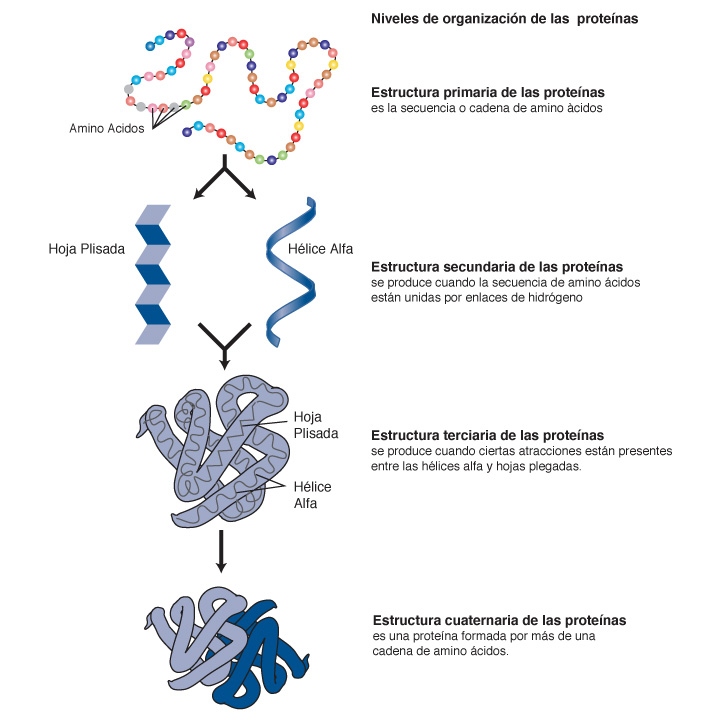
\includegraphics[scale=.6]{images/protein_lg.jpg}
	\caption{\em Niveles estructurales de la proteína (\citealp{image:genome-project})}
	\label{fig:structures-protein}
\end{figure}

\subsubsection{Estructuras Primarias y el Dogma de Anfinsen}
La estructura primaria de la proteína se define como el conjunto ordenado de aminoácidos dispuestos en forma de secuencia, a partir de la cual, tras la etapa de plegamiento (más detalle en la sección \ref{fundamentos:plegamiento}), se consolida la estructura a nivel funcional. Esto último se conoce como el \textit{Dogma de Anfinsen} (\citealp{Anfinsen:1973}) o \textit{Hipótesis de la termodinámica}. Por ejemplo, la proteína cuyo \textit{Protein Data Bank ID (PID)} es \textit{1K43} (\citealp{1k43}), tiene un largo de 14 aminoácidos, su estructura primaria viene dada por la representación lineal \textit{RGKWTYNGITYEGR}.

\subsubsection{Estructuras Secundarias y Clasificaci\'on STRIDE}
\label{cap:dssp}

Esta conformación molecular se forma por la presencia de patrones de enlaces de hidrógeno entre los átomos del grupo amino y carboxilo del polipéptido.

La organización estable de residuos de una proteína forman tipos de estructuras que son identificables. La formación de estas estructuras neutraliza los grupos polares en cada aminoácido. En el núcleo de la proteína las estructuras secundarias tienen un espacio limitado por lo que se encuentran cercas una de otra, debido a esto, el grupo lateral de cada aminoácido puede reaccionar con el de otro residuo. Esto es un factor a considerar en el modelado y alineamiento molecular (\citealp{molecular:book}).

Cuando se habla de estructuras secundarias de proteína, usualmente se usa la clasificación del código STRIDE que clasifica estas estructuras en 8 estados conformacionales (\citealp{stridepaper}).

%El código DSSP es el método estándar para asignar estructuras secundarias a los aminoácidos de la proteína y se basa en la detección de patrones de enlaces de hidrógeno, esta técnica fue inicialmente propuesta por \citealp{pauling:1951}. 

El funcionamiento de este algoritmo comienza por identificar los enlaces de hidrógeno implicados en la cadena principal (cadena de átomos enlazados con enlaces peptídicos) usando solamente su definición electrostática, asumiendo cargas parciales de \textit{-0.42e} y \textit{+0.20e} para el oxígeno del grupo carbonilo y el hidrógeno del grupo amida respectivamente. Los valores opuestos a estos son asignados al carbono del grupo carbonilo y al nitrógeno del grupo amida. Un enlace de hidrógeno es detectado si \textit{E} en la ecuación \ref{equation:ene-h} es menor que $-0.5kcal/mol$. 
\begin{equation}
	E=0.084*(\frac{1}{r_{ON}}+\frac{1}{r_{CH}}+\frac{1}{r_{OH}}+\frac{1}{r_{CN}})*332\frac{kcal}{mol}
	\label{equation:ene-h}
\end{equation}

Basado en esto, ocho tipos de estructuras secundarias pueden ser asignadas (ver tabla \ref{table:dssp}). La clasificación STRIDE establece un mínimo de residuos que participan en cada una de las estructuras secundarias. Por ejemplo, las conformaciones tipo hélices (G,H e I) y hojas requieren al menos 3.6 residuos adyacentes que deben formar parte del mismo patrón de enlaces de hidrógeno. Si la hélice u hoja es muy corta será designada como T o B respectivamente.

\begin{table}[h]
    \caption{Clasificaci\'on STRIDE y códigos asociados}
	\centering
	\begin{tabular}{|r|l|}
		\hline
		\textbf{Nombre estructura secundaria} & \textbf{Código STRIDE} \\ \hline
		$3_{10}$-helix 	& G		\\		
		$\alpha$-helix 	& H		\\ 		
		$\pi$-helix 	& I		\\  	
		$\beta$-bridge 	& B		\\ 		
		$\beta$-bulges 	& E		\\ 		
		Turn 			& T		\\		
		Bend 			& S		\\	
		Coil 			& C		\\		\hline
	\end{tabular}
	\label{table:dssp}
\end{table}


Para una simplificación de la definición, las 8 estructuras se pueden generalizar en cuatro:


\begin{itemize}
	\item \textbf{\textit{Hélices (Helix)}:} Las hélices ($3_{10}$-helix, $\alpha$-helix y $\pi$-helix ) corresponden al tipo más abundante de estructura secundaria. Las hélices tienen 3.6 aminoácidos por vuelta con un enlace de Hidrógeno formado cada 4 residuos; la longitud media es de 10 aminoácidos, no obstante, varía de 5 a 40 residuos por hélice (\citealp{molecular:book}). La alineación de los enlaces de H crea un momento dipolar de la hélice con una carga parcial positiva resultante en el extremo amino de esta. Debido a que esta región cuenta con grupos NH2 libres, puede interactuar con grupos cargados negativamente, tales como los fosfatos. La localización más frecuente de las hélices está en la superficie del núcleo de la proteína, proporcionando una interfaz con el entorno acuoso. La cara interna de la hélice tiende a tener aminoácidos hidrofóbicos, mientras que la cara externa tiende a ser hidrofílica. Por lo tanto, un tercio de 4 aminoácidos de la cadena tenderá a ser hidrofóbico, este patrón se puede detectar con bastante facilidad. Por ejemplo, las hélices a inmersas en el núcleo de la proteína o en las membranas celulares tienen una distribución más alta y regular de aminoácidos hidrofóbicos, por lo tanto, se pueden detectar y predecir con alta precisión. Las hélices expuestas en la superficie tienen una menor proporción de aminoácidos hidrofóbicos. Regiones con alta presencia de alanina, ácido glutamínico, leucina, metionina y baja de prolina, glicina, tirosina, serina tienden a formar una una hélice (\citealp{lehninger}).
	
	\begin{figure}[H]
		\centering
		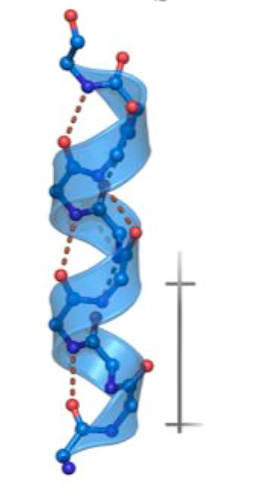
\includegraphics[scale=.4]{images/helix.png}
		\caption{\em Ejemplo de Hélice (pág. 25, \citealp{bioinfopt}).}
		\label{fig:helix}
	\end{figure}

	
	\item \textbf{\textit{Hojas (Sheets)}:} Las hojas se forman por enlaces de Hidrógeno entre un promedio de 5-10 aminoácidos consecutivos en una porción de la cadena con otra porción de 5-10 más abajo de la cadena. Las regiones que interactúan pueden ser adyacentes, con un lazo corto entre estas, o muy separados, con otras estructuras secundarias en  medio (\citealp{lehninger}). Cada hebra puede ir en la misma dirección para formar una hoja paralela, sin embargo, pueden tener dirección inversa para formar una hoja anti-paralela, o pueden estar mezcladas hojas paralelas con anti-paralelas para generar una hoja más compleja y mixta, ver figura \ref{fig:beta-sheets}. Cada aminoácido en las hebras interiores de la hoja forma dos enlaces de Hidrógeno con aminoácidos vecinos, mientras que cada aminoácido en las hebras externas forma solamente un enlace con la hebra interior (\citealp{molecular:book}).
	
	\begin{figure}[H]
		\centering
		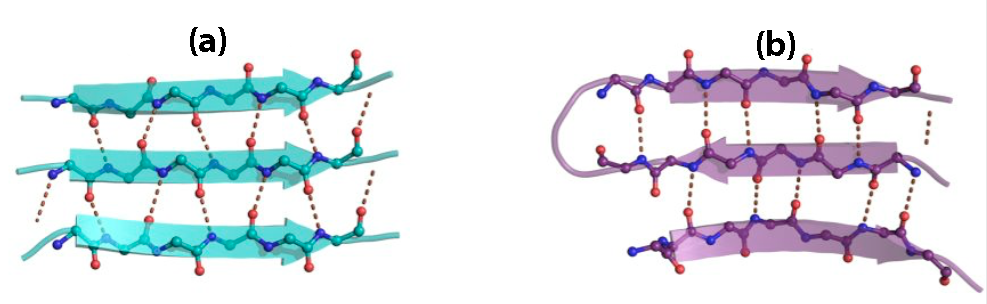
\includegraphics[scale=0.45]{images/beta.png}
		\caption{\em Ejemplo de \textbeta-hojas (a) paralela y (b) antiparalela (pág. 25, \citealp{bioinfopt}).}
		\label{fig:beta-sheets}
	\end{figure}

	\item \textbf{\textit{Vueltas (Turns)}:} Las vueltas son regiones de una cadena que se encuentran entre las hélices y hojas, de diferentes longitudes y configuraciones tridimensionales. Las vueltas en forma de U representan una vuelta completa en la cadena de polipéptido que une dos hebras (anti-paralelas o paralelas) y pueden ser tan cortas como dos aminoácidos de longitud (\citealp{molecular:book}).
	\begin{figure}[H]
		\centering
		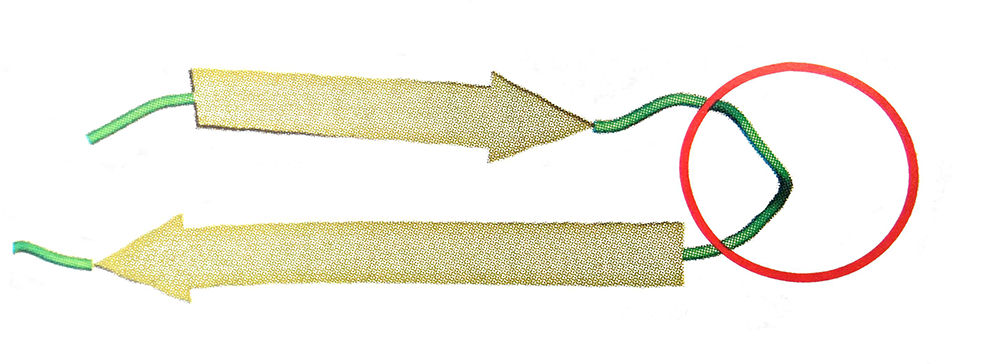
\includegraphics[scale=.8]{images/turn.png}
		\caption{\em Ejemplo de vuelta que se forma entre dos $\beta$-hojas (pág. 136, \citealp{book:kessel}).}
		\label{fig:turns}
	\end{figure}
	
	\item \textbf{\textit{Bobinas (Coils)}:} Las bobinas son aquellas secciones de la cadena de la proteína que no pueden ser clasificadas como hélices, hojas o vueltas (\citealp{molecular:book}).
\end{itemize}

%El código DSSP es una simplificación de la continuas variaciones de los patrones de enlaces de Hidrógeno presentes en una proteína. La mayoría de los métodos de predicción de estructuras secundarias simplifica aún más, llegando a una clasificación de 3 estructuras: hélices, hojas y bobinas. Los primeros métodos de predicción de estructuras secundarias estaban basados en cuán propenso era un aminoácido de formar parte de una hélice u hoja. Dichos métodos tenían una precisión del 60\% en la predicción de estos tres estados conformacionales (\citealp{Finkelstein:1971}). Al usar redes neuronales y máquinas vector de soporte, la precisión alcanzó valores mayores al 70\% (\citealp{Rost:1993}). Métodos posteriores logran hasta un 80$\sim$90\% de acierto (\citealp{Dor:2007}). La precisión de las predicciones de las estructuras secundarias juega un papel fundamental, ya que existen variados métodos que usan esta información como puntapié inicial para comenzar la predicción de las estructuras terciarias.

\subsubsection{Estructuras Terciarias}
\label{fundamentos:estructura-terciaria}

La estructura terciaria de la proteína tiene solo una cadena principal de aminoácidos y su principal característica es que se considera la posición espacial de cada átomo de la estructura (\citealp{branden:1999}). Puesto que se tiene esta información, se puede afirmar que la estructura terciaria corresponde al estado mínimo funcional de la proteína de la que se puede extraer conclusiones de sus propiedades biológicas, a través de su capacidad para interactuar con moléculas de otras proteínas o grupos celulares (\citealp{molecular:book}).

Esta estructura está compuesta por la unión de varias estructuras secundarias, que debido a interacciones que se mencionan posteriormente, se pliegan y distribuyen en el espacio dando forma al péptido. En la estructura terciaria, comúnmente los aminoácidos apolares se sitúan hacia el interior de la proteína, mientras que los polares hacia el exterior, lo que posibilita la interacción con los átomos de agua del medio acuoso. Por ejemplo, las proteínas integrales de membrana poseen a sus aminoácidos hidrofóbicos en la cara interna de la bicapa lipídica. Por lo tanto, la polaridad o apolaridad de los aminoácidos y su disposición influyen en las propiedades físico-químicas de la proteína (\citealp{branden:1999}).

\begin{figure}[H]
	\centering
	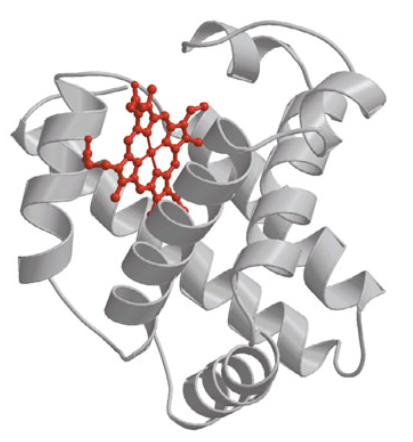
\includegraphics[scale=.5]{images/terciaria.png}
	\caption{\em Ejemplo de estructura terciaria: Mioglobina (pág. 133, \citealp{lehninger}).}
	\label{fig:ter-struct}
\end{figure}

Las interacciones que ocurren en la estructura terciaria de la proteína son cuatro (\citealp{branden:1999}):
\begin{itemize}
	\item Enlaces puentes de disulfuro entre Cistinas.
	\item Puentes de hidrógeno entre las cadenas laterales.
	\item Fuerzas e interacciones de \textit{van} der Waals.
	\item Efecto hidrofóbico de las móleculas.
\end{itemize}

Estas interacciones deben ser consideradas en la determinación y predicción de la estructura terciaria. Tal como se mencionó en la sección \ref{intro:enunciado}, este trabajo se concentra en la predicción de la proteína en su estructura terciaria. Los métodos experimentales más usados que dan información de la conformación de estos estados funcionales son los siguientes:

\begin{itemize}
	\item \textbf{Interferometría de doble polarización:} Este método se concentra en obtener información de la superficie de estas estructuras para determinar y monitorear los cambios conformacionales que sufre la proteína \cite[Cap.\ 11]{bioinfopt}.
	\item \textbf{Resonancia magnética nuclear:} Si bien, no provee una alta precisión como el método anterior, si puede indicar los cambios conformacionales que tiene una proteína en el medio \cite[Cap.\ 12]{bioinfopt}.
	\item \textbf{Cristalografía por rayos X:} Es la técnica más usada para determinar la estructura de la proteína. Provee información precisa del estado tridimensional pero no acerca de la flexibilidad conformacional \cite[Cap.\ 13]{bioinfopt}.
	
\end{itemize}

\subsubsection{Estructuras Cuaternarias}
Las estructuras cuaternarias son aquellas que poseen más de una cadena principal de polipéptidos, es decir, es la unión de dos o más estructuras terciarias (\citealp{branden:1999}), por lo que tienden a ser complejas estructuras funcionales.

Estas estructuras son de vital importancia biológica, ya que en base a ellas se realiza la construcción celular de, por ejemplo, microtúbulos, microfilamentos, capsómeros de virus y complejos enzimáticos que pueden activar o inhibir funciones biológicas (\cite[Cap.\ 4.3]{lehninger}). 

\subsection{Plegamiento de proteínas}
\label{fundamentos:plegamiento}

El plegamiento de proteínas (en inglés \textit{Protein folding}) es el proceso por el cual una proteína alcanza su estructura espacial. Como ya se ha mencionado, la estructura tridimensional marca las funcionalidades a nivel biológico (\citealp{Alberts:2002}), por lo que un incorrecto plegamiento implicaría una proteína inactiva o tóxica.

\begin{figure}[h]
	\centering
	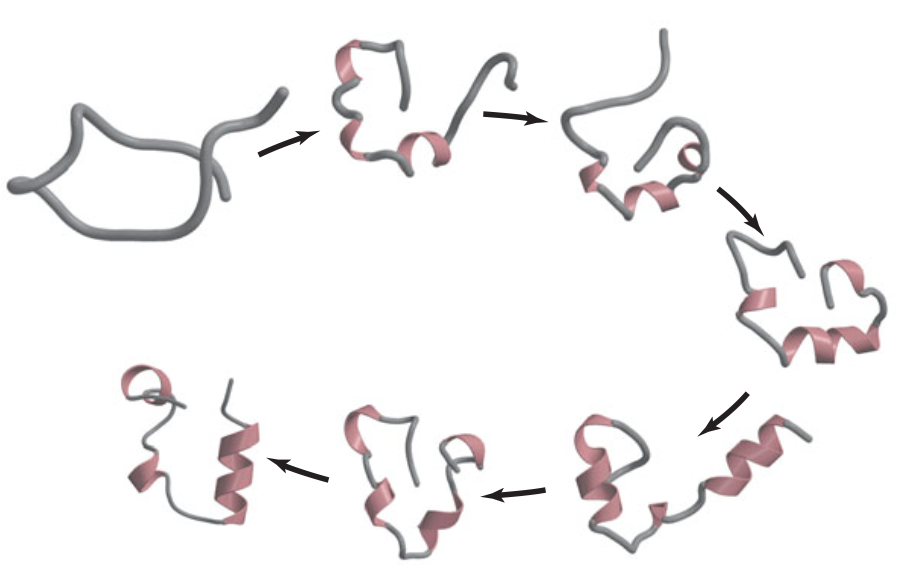
\includegraphics[scale=.5]{images/folding.png}
	\caption{\em Plegamiento de proteína (pág. 142, \citealp{lehninger}).}
	\label{fig:protein-folding}
\end{figure}

El proceso inverso al plegamiento se conoce como desnaturalización de proteínas. Una proteína que sufre este proceso deja de ser funcional al no tener una estructura tridimensional estable y definida. 

El plegamiento de la proteína se debe principalmente al medio en el que se encuentra y a los propiedades de los átomos y moléculas que la conforman. A medida que la proteína se pliega, pasa por etapas de plegamiento que asumen cambios en la energía global del sistema o estructura. Las variaciones energéticas se deben a factores termodinámicos como la entropía conformacional, los puentes de hidrógeno, las interacciones hidrofóbicas e hidrofílicas, y las interacciones de \textit{van} der Waals (\citealp{folding}). A continuación se definen brevemente estos conceptos.

\subsubsection{Entropía conformacional}

La conformación nativa de una proteína es la conformación de más baja energía libre de Gibbs. El proceso de plegamiento, como cualquier otro proceso biológico, se encuentra bajo control termodinámico y cinético, y es un proceso que está claramente favorecido en condiciones naturales. En otras palablas, el proceso de plegamiento hasta alcanzar la estructura nativa presenta un $\Delta$G negativo. Desde el punto de vista entrópico, el proceso de plegamiento supone una disminución neta de entropía desde la estructura denominada ovillo aleatorio (cuando la proteína está sin forma definida) a la única estructura nativa (estructura funcional). Este descenso de entropía, denominada entropía conformacional, supone un incremento positivo de energía libre en el proceso de plegamiento ($\Delta G = \Delta H – T\Delta S$). Para poder tener un descenso global en el proceso es necesario que el incremento de entalpía ($\Delta H$) sea negativo o que existan otros aumentos de entropía ($\Delta S$). La principal contribución entalpica al proceso de plegamiento la constituyen la formación de interacciones no covalentes que estabilizan la estructura nativa y las interacciones hidrofóbicas entre las cadenas laterales apolares que generalmente están localizadas al interior de la proteína (\citealp{entropia}).

\subsubsection{Enlaces de hidrógeno internos}

Un enlace de hidrógeno es la fuerza atractiva entre un átomo con carga negativa y un átomo de hidrógeno unido mediante un enlace covalente a otro átomo negativo, ver figura \ref{fig:h-bond}. 
\begin{figure}[h]
	\centering
	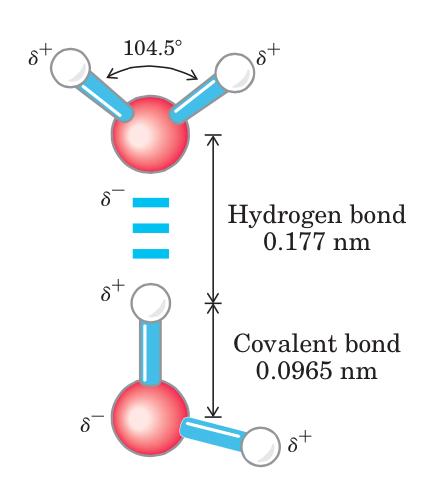
\includegraphics[scale=.5]{images/hidrobond.png}
	\caption{\em Enlace de hidrógeno (pág. 44, \citealp{lehninger}).}
	\label{fig:h-bond}
\end{figure}

Los patrones que forman estos enlaces  son lo usados por distintos métodos para poder predecir estructuras secundarias, actúan como estabilizadores lo que ayuda a la estructura terciaria a mantenerse definida (\citealp{hbond}).

\subsubsection{Fuerzas o Interacciones de \textit{van} der Waals}
Las fuerzas de \textit{van} der Waals son las fuerzas atractivas o repulsivas entre moléculas y/o átomos. Cuando se encuentran a una distancia moderada, las moléculas se atraen entre si, pero cuando sus nubes electrónicas empiezan a sobreponerse, las moléculas se repelen con fuerza (\citealp{entropia}). Ver gráfico figura \ref{fig:graph-vanderwaals}.
\begin{figure}[h]
	\centering
	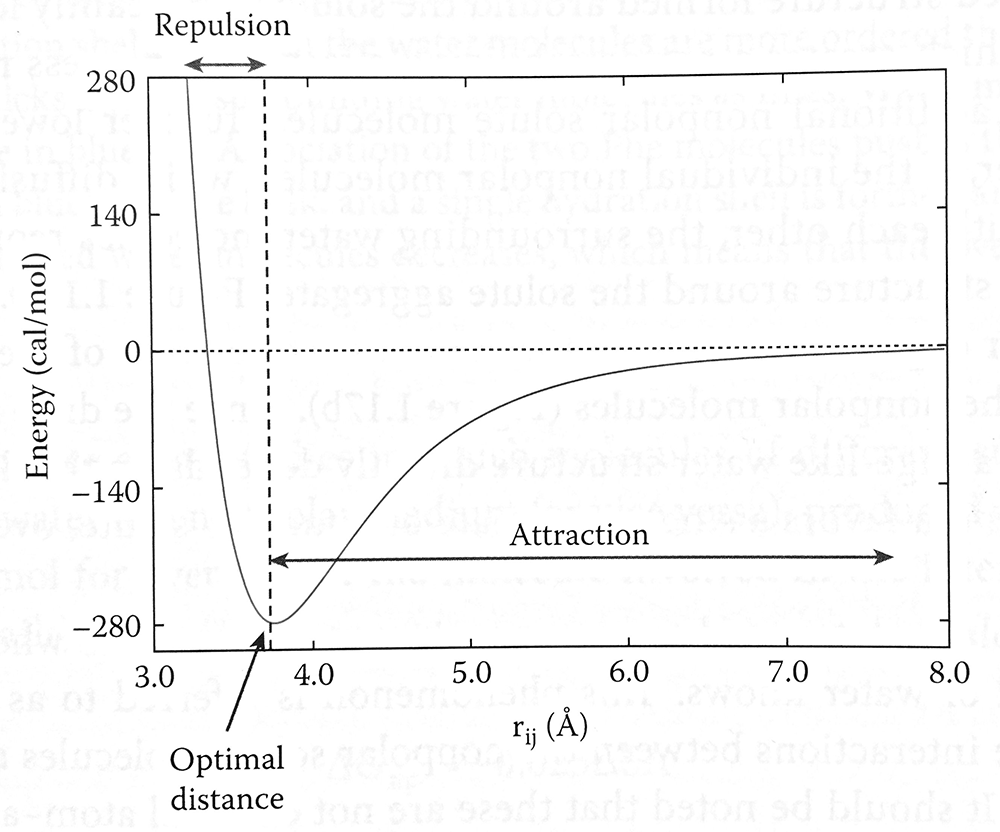
\includegraphics[scale=1]{images/vanderwaals.png}
	\caption{\em Gráfico de energía versus distancia entre átomos (pág. 55 \citealp{book:kessel}).}
	\label{fig:graph-vanderwaals}
\end{figure}

\subsubsection{Interacciones hidrofóbicas}

Toda sustancia hidrofóbica en contacto con moléculas de agua provoca fuerzas repulsivas produciéndose una separación entre estas. En el caso de las proteínas, los aminoácidos hidrofóbicos de las estructuras terciarias tienden a estar hacia el núcleo del polipéptido, lo que contribuye a un aumento de la entropía conformacional y a la estabilidad de la estructura al disminuir fuerzas repulsivas que generen cambios espaciales de los átomos  (\citealp{molecular:book}).

Luego de revisar los conceptos anteriores, se puede vislumbrar que minimizar el número de átomos o moléculas hidrofóbicas de la cadena lateral que están expuestas al agua, constituye una importante fuente de estabilización en el proceso de plegado. Además, la formación de enlaces de hidrógenos a nivel intramolecular de la proteína permite aumentar la estabilidad de la estructura, sin olvidar que la fuerza de estos enlaces de hidrógeno dependen del medio en el que se encuentran, de modo que, serán más fuertes si se encuentran en un medio hidrofóbico que en un medio hidrofílico (\citealp{molecular:book}).

\subsection{Campos de fuerza}

En el área de la Dinámica Molecular (\citealp{Karplus10052005}), un campo de fuerza se refiere al modelo de funciones matemáticas utilizadas para describir la energía potencial de un sistema de átomos y moléculas. Las funciones de campo de fuerza y el conjuntos de parámetros usados se derivan tanto del trabajo experimental y de cálculos de mecánica cuántica. Existen variados campos de fuerza propuestos por el mundo de la bioquímica y biofísica, pero para el presente trabajo se mencionará solo los campos \textit{Coarse grained}, que son los más utilizados en las predicciones de las proteínas, tienen la ventaja de representar mejor el medio y contexto en el que se desenvuelve la macro-molécula, por lo que proporcionan representaciones más fidedignas, esto aumenta la efectividad computacional (\citealp{hornak:2006}).

\subsubsection{Forma general de un campo de fuerza}

La forma de una campo de fuerza envuelve todos elementos unidos por enlaces (\textit{bonded terms}), que son aquellos átomos que están enlazados mediante enlaces covalentes, y los términos no enlazados (\textit{nonbonded terms}) que corresponden en su mayoría a fuerzas electrostáticas y de \textit{van} der Waals. Cada campo de fuerza tiene su propia fórmula matemática, pero se pueden generalizar de la siguiente forma.
\begin{equation}
	E_{total}=E_{bonded}+E_{nonbonded}
\end{equation}

donde:
\begin{equation}
E_{bonded}=E_{bond}+E_{angle}+E_{dihedral}
\end{equation}
\begin{equation}
\label{eq:nonbonded}
E_{nonbonded}=E_{electrostatic}+E_{van der waals}
\end{equation}

\subsubsection{Parametrizaciones de los campos de fuerza}

Cada campo de fuerza posee y se define con un conjunto de parámetros por cada tipo de átomo. Por ejemplo, un campo de fuerza podría tener distintos parámetros para un átomo de oxígeno en un grupo carbonilo y un grupo hidroxilo. Los parámetros más comunes incluyen la mása del átomo, el radio de \textit{van} der Waals y la carga parcial para los átomos, los valores correspondientes al largo de los enlaces, ángulos de estos y ángulos de torsión para pares, tripletas y cuadripletas de átomos enlazados. Los campos de fuerza más usados poseen cargas parciales fijas para los átomos debido que consideran que la electroestática del medio no interfiere en su carga. No obstante, se están desarrollando campos de fuerza que proponen la polarización de los átomos a causa de sus átomos vecinos (\citealp{Beauchamp:2012}).

\subsubsection{Deficiencias}

Todos los campos de fuerza se basan en aproximaciones numéricas derivadas de diferentes tipos de datos experimentales. Algunos de los campos de fuerza no contemplan la polarización del entorno, un efecto que puede reducir significativamente las interacciones electroestáticas sobre la carga parcial de los átomos (\citealp{hornak:2006}). Además, las fuerzas de \textit{van} der Waals están altamente ligadas al ambiente de la simulación, debido a las fuerzas que se originan de las interacciones de dipolos inducidos e instantáneos producidos entre el ambiente acuoso y las moléculas del péptido. 

Lo revisado anteriormente indica que la alta parametrización empírica provoca limitaciones de las simulaciones, produciendo sesgos y pérdida de precisión.

\subsection{Estado del Arte}
\label{fundamentos:estado-arte}

El foco de este trabajo está en el marco de predicción de estructuras terciarias de proteínas. En consecuencia, el estado del arte presentado da una visión general de las principales soluciones y técnicas usadas hoy en día para llevar a cabo dicho objetivo. Además, cabe mencionar los métodos actuales usados en la predicción de estructuras secundarias, ya que la solución propuesta en este trabajo hace uso de esa información.

Como dato adicional, cada dos años se realiza un experimento comunitario mundial llamado \text{\textit{CASP}} (\textit{Critical Assessment of Techniques for Protein Structure Prediction, Evaluación crítica de las técnicas para la predicción estructural proteica}) cuya función es dar a conocer métodos actuales de predicción y proveer una forma objetiva de evaluación de estos métodos (\citealp{casp:1995}). 

\subsubsection{Determinación de estructuras secundarias}

Uno de los primeros algoritmos propuestos en los años 70 fue el método de \textit{Chow-Fasman} \citealp{fasman:1974}, el cual se basa en la probabilidad de un residuo de pertenecer a cada tipo de estructura secundaria. Este algoritmo producía resultados con una precisión del 50$\sim$60\%, la baja precisión se debe a la cantidad de reducida de información disponible en esa época. Unos años más tarde, el método de GOR (\citealp{garnier:1978}) permitía obtener una precisión del 60 a 65\% al incorporar al algoritmo de Chow-Fasman la influencia de los residuos vecinos en la probabilidad de formar una cierta estructura secundaria. El siguiente avance significativo viene con el uso de redes neuronales (\textit{Neural Networks, NN}) y máquinas vector de soporte (\textit{Support Vector Machine, SVM}) aumentaron la precisión por sobre el 70\% (\citealp{Rost:1993}) llegando a alcanzar el 90\% (\citealp{Dor:2007}). En la actualidad gracias a internet, es posible acceder a herramientas tipo NN como \textit{PSIPRED SERVER} (\citealp{psipred:2013}) basado en el algortimo \textit{PSIBLAST} (propuesto en \citealp{psiblast:1997}) alcanzando una precisión de 81.6\%, y \textit{JPRED 3 SERVER} (\citealp{jpred:2008}) que hace uso del algoritmo \textit{JNET} (\citealp{jpred:2000}) con un 81.5\%. Para determinar las estructuras secundarias de las proteínas usadas en este trabajo, se hace uso de STRIDE (\citealp{stride:2004}) el cual fue revisado en la sección \ref{cap:dssp}.

\subsubsection{Predicción de estructuras terciarias}

La predicción de estructuras terciarias continua siendo un problema de extrema dificultad. Los dos principales problemas de la simulación es el cálculo de la energía libre de la proteína y función de minimización de energía. Los métodos de predicción deben explorar el espacio de soluciones para encontrar la estructura que cumple los requisitos planteados anteriormente, el problema recae en el espacio de búsqueda que resulta ser muy amplio a medida que la cadena de residuos aumenta, lo que hace intratable el problema debido al costo computacional que conlleva. Estos problemas pueden ser aminorados parcialmente usando técnicas de modelado por homología y enhebrado de secuencias, cuyo fundamento se basa en asumir que si se tiene la estructura generada de una secuencia, al tener la misma secuencia en otra proteína tenderá a formar una estructura similar (\citealp{Zhang:2008}).

Los enfoques actuales para predecir la estructura terciaria de la proteína según son cuatro (\citealp{Dorn2014251}), planteados a continuación.

\subsubsection{Métodos ab initio sin información de bases de datos}
Los métodos \textit{ab initio} o \textit{de novo} son técnicas de modelamiento que buscan construir la estructura tridimensional de la proteína simulando los procesos termodínamicos que ocurren a nivel biológico (\citealp{floudas:2006}). Intentan reproducir el comportamiento y las etapas de plegado de la proteína mediante la minimización de la energía libre del sistema haciendo uso de eventos moleculares. A medida que la cantidad de residuos aumenta, la cantidad de recursos computacionales necesarios en este método se incrementa debido a la complejidad del problema (\citealp{Crescenzi:1998}). Se han creado supercomputadoras específicamente para resolver este problema usando métodos \textit{ab initio}, como \textit{BLUE GENE} (\citealp{bluegene:2001}) y \textit{MDGRAPE-3} (\citealp{mdgrape:2003}) o amplias estructuras distribuidas, como el proyecto \textit{ROBETTA} (\citealp{robetta}).

\subsubsection{Métodos ab initio con información de bases de datos}
\label{fundamentos:abinitio-db}
Los métodos basados en \textit{ab initio} que utilizan información de base de datos son una variante del método anterior, ya que la principal diferencia radica en que usan información experimental para crear una estructura inicial más acabada, pudiendo ser refinada usando técnicas de Dinámica Molecular \citealp{floudas:2006}. Algunos de los métodos actuales son \textit{I-TASSER} (\citealp{itasser:2015}), \textit{ANGLOR} (\citealp{anglor:2008}) y \textit{FRAGFOLD} (\citealp{fragfold:2001}) y \textit{ROSETTA} (\citealp{rosseta:2010}).


\subsubsection{Métodos de enhebrado}
Estos métodos usan la alineación de secuencia con una base de datos para obtener estructuras conocidas que después irán uniendo a la predicción (\citealp{floudas:2006}). El principal problema de esta técnica es la búsqueda de secuencias en las bases de datos, ya que una secuencia de una estructura puede estar presente en las bases de datos experimentales más de una vez y con distintas conformaciones espaciales. Otro problema ligado a las técnicas de alineación es el largo de la secuencia a buscar, ya que al aumentar, las posibles combinaciones de sub-secuencias crece de manera considerable (\citealp{lathrop:1994}). Herramientas disponibles de esta área son \textit{GENTHREADER} \citealp{genthreader:1999}, \textit{PROSPECT} \citealp{kim:2003} y \textit{HHpred} (\citealp{soding:2005}).


\subsubsection{Métodos de modelado por comparación}
Los métodos de modelado por comparación se basan en el principio de que las estructuras secundarias se conservan más evolutivamente que las secuencias de aminoácidos que las generan (\citealp{floudas:2006}). Por  ejemplo, si se tiene una estructura secundaria tipo hélice con 10 residuos, el método buscará en las bases de datos hélices con una cantidad de residuos similar (sin importar cuales sean), y mediante una función de fitness escogerá la mejor estructura tridimensional para la predicción. Ejemplos de este método son \textit{MODELLER} (\citealp{eswar:2002}), \textit{CLUSTALW} (\citealp{clustalw}) y \textit{COMPASS} (\citealp{compass}).

\section{Algoritmos meméticos}

En el mundo de la informática, existen métodos de resolución de problemas de optimización que permiten encontrar soluciones cercanas al óptimo global (mínimo o máximo según corresponda), estos métodos son llamados metaheurísticas y son usados generalmente cuando el problema no puede ser resuelto con métodos tradicionales ya que las implementaciones pueden ser impracticables y demasiado costosas a nivel computacional. Dentro de este conjunto de técnicas se encuentran los algoritmos meméticos.

\label{fundamentos:memeticos}

\subsection{Definición}
Un algoritmo memético (\textit{Memetic Algorithm, MA}) es una metaheurística evolutiva basada en población que usa un operador de búsqueda local para el refinamiento de sus soluciones (\citealp{moscato:2011}). El nombre proviene de la palabra \textit{meme} la que puede entenderse como un objeto cultural que es transmitido por repetición y replicación de manera análoga a la transmisión biológica de genes (\citealp{meme:2015}).

\subsection{Estructura}

El algoritmo \ref{alg:memetico-gen} muestra la estructura general de un MA genérico. Los algoritmos meméticos están compuestos por operadores evolutivos más un operador de búsqueda local. Estos operadores actúan sobre agentes que componen la población, esta es la principal diferencia con los algoritmos evolutivos que hacen uso de individuos. La diferencia entre individuo y agente radica en que el primero es un ente pasivo que está sujeto a procesos y reglas evolutivas, mientras que un \textit{agente} es un ente activo que busca mejorar haciendo uso de la información propia del problema (a través de la búsqueda local) (\citealp{moscato:2011}).

En primer lugar, los algoritmos meméticos deben inicializarse con una población inicial de soluciones (lineas 2 al 5, algoritmo \ref{alg:memetico-gen}), que generalmente son obtenidas por funciones aleatorias, lo que deja de manera implícita que no se preocupan de la calidad ni eficiencia de la solución. Una vez que se tiene la base de la población sobre la cual se va a iterar, (cada iteración sobre la población se conoce como generación) se realiza el ciclo generacional para hacer evolucionar el sistema (lineas 7 al 25, algoritmo \ref{alg:memetico-gen}) o converger a soluciones prometedoras que sean iguales o cercanas al óptimo global del problema en cuestión (\citealp{hugo}). Las líneas 10 al 13 corresponden a la etapa de cruzamiento, en esta se escogen las soluciones a cruzar. Luego, la línea 14 muestra la acción del operador de búsqueda local, esta etapa es vital en los algoritmos meméticos por definición, ya que es en donde se aplica el conocimiento acerca del problema para conducir a mejores soluciones. Posteriormente, continua la etapa de mutación que brinda de diversidad a la población y permite escapar de mínimos locales (lineas 16 al 18, algoritmo \ref{alg:memetico-gen}). Los criterios de fin de las generaciones pueden ser variados, a modo de ejemplo, se puede elegir que termine cuando se alcanzan 100 generaciones o que el tiempo de ejecución sea de 10 horas.

\begin{algorithm}[ht]
	\begin{algorithmic}[1]
		\REQUIRE una instancia \textit{I} de un problema \textit{P}
		\ENSURE una solución \textit{sol}
		\STATE		\COMMENT Población inicial
		\FOR {$j \leftarrow 1:popsize$}
		\STATE $ind \leftarrow $GenerarSol(\textit{I})
		\STATE $pop[j] \leftarrow$ MejoraLocal(\textit{ind})
		\ENDFOR
		\STATE \COMMENT Ciclo Generacional
		\REPEAT
		\STATE \COMMENT etapa de reproducción o cruzamiento
		\FOR {$j \leftarrow 1:popsize$}
		\STATE $padres \leftarrow$ SeleccionarPadres(\textit{pop})
		\STATE $newind \leftarrow$ Cruzamiento(\textit{padres})
		\STATE $newpop[j] \leftarrow newind$
		\STATE \COMMENT etapa de búsqueda local
		\STATE $newpop[j] \leftarrow$ MejoraLocal(\textit{newpop[j]})
		\STATE \COMMENT etapa de mutación
		\IF{probmutar() == \TRUE}
		\STATE $newpop[j] \leftarrow$ mutar(\textit{newpop[j]})
		\ENDIF
		\ENDFOR
		\STATE \COMMENT etapa de actualización de la población
		\STATE $pop \leftarrow $ActualizarPop(\textit{pop,newpop})
		\IF{ConvergenciaPop(pop) == \TRUE}
		\STATE $pop \leftarrow$ reiniciarPop(pop)
		\ENDIF
		\UNTIL CriterioFin(\textit{pop})
		\RETURN MejorSol(\textit{pop})
	\end{algorithmic}
	\caption{Algoritmo memético general}
	\label{alg:memetico-gen}
\end{algorithm}

Como los algoritmos meméticos son algoritmos evolutivos, los operadores de reproducción y mutación tienen la misma estructura, puede variar el operador de cruzamiento de manera de detectar patrones que se repiten a lo largo de la población y que podría representar una convergencia evolutiva deseable, un \textit{meme} que se desea preservar. Por último, la actualización de la población dependerá de la estructura y reglas evolutivas que tenga la población (\citealp{Buriol:2004}). Por ejemplo, se puede tener una estructura jerárquica de población o una estructura de castas en base al \textit{fitness} del agente, en la que se preservará el 30\% de los mejores agentes y el 70\% restante se reiniciará con nuevas soluciones aleatorias. Finalmente, una vez terminado el ciclo generacional, se retorna el mejor agente de la población (basado en el \textit{fitness} de la solución y del tipo de optimización).

\newpage
\chapter{Dise\~no e implementaci\'on de la soluci\'on}
\label{cap:diseno}

Esta etapa contempla el diseño de la solución correspondiente a un algoritmo memético (\textbf{MA}) para predecir la estructura terciaria de la proteína.

\section{Algoritmo memético para el problema 3-D PSP}

Como se revisó en la sección \ref{fundamentos:memeticos}, los algoritmos meméticos son algoritmos evolutivos que aprovechan toda la información disponible para mejorar los agentes de la población, de forma activa mediante el uso de búsqueda local.

También, el enfoque que adopta el MA es el visto en la sección \ref{fundamentos:abinitio-db}, ya que se usará la función de energía potencial \textit{Amber Force Field 14 SB} (versión actualizada de \textit{Amber Force Field 99 SB}, \citealp{amber14}) como función de minimización. El conocimiento biológico que usa el MA para generar sus agentes y modificarlos, viene dado por lo observado experimentalmente en la naturaleza, esta información está almacenada en la \textit{Protein Data Bank}. 
 
Para hacer uso de esta información a nivel algorítmico se debe crear una estructura que indique cuáles son los ángulos más probables para un aminoácido según la estructura secundaria en la que se encuentra. Por ejemplo, si el residuo Alanina está dentro de una $\alpha$-helix, el método debe escoger con una alta probabilidad los ángulos de torsión que más usa este residuo para formar dicho estado conformacional. Para realizar esta elección de ángulos se usará la \textit{Lista de ángulos de probabilidades de ocurrencia \textbf{APL}} desarrollada en \citealp{Dorn:2013} y que está explicada a continuación.

\subsection{Lista de ángulos de probabilidades de ocurrencia APL}
Este algoritmo toma ventaja del conocimiento experimental almacenado en la Protein Data Bank (\citealp{Berman:2000}). Los pares de ángulos $\phi$ y $\psi$ pueden tomar valores reales entre $-180º$ y $180º$. En consecuencia, el espacio de búsqueda por cada residuo es astronómicamente amplio y la complejidad del problema aumenta según se incremente la cantidad de residuos. No obstante, si se visualiza la información almacenada en la PDB se ve que los diferentes residuos tienen diferentes distribución de ángulos. En la figura \ref{fig:rmc-glicina} se puede observar que los pares de ángulos más usados están en dos regiones representadas por el área de color más oscuro.

\begin{figure}[H]
	\centering
	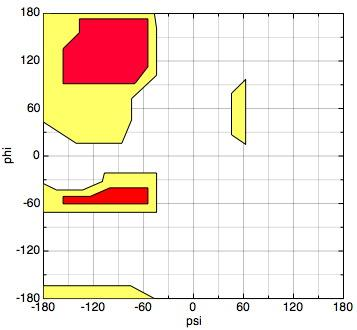
\includegraphics[scale=.5]{images/rama-plot.jpg}
	\caption{\em Ejemplo de mapa de Ramachandran para los ángulos \textphi~y~\textpsi~de un amino\'acido (pág. 105 \citealp{book:kessel}).}
	\label{fig:rmc-glicina} 
\end{figure}

La gran ventaja de incorporar esta información al algoritmo memético es poder reducir el espacio de búsqueda de soluciones, mediante la asignación de probabilidades de selección de ángulos según su ocurrencia experimental.

Para incluir esta información se construirá un histograma \textit{$H_{a,z}$} de $361{\times}361$ celdas para cada residuo de aminoácidos \textit{a} con estructura secundaria \textit{z}. Cada celda $(i,j)$ tendrá el número de veces que el par \textit{(a,z)} ha tenido esa coordenada presente. En orden de incrementar la representación de las áreas más densas, los valores de las 8 celdas adyacentes a $(i,j)$ serán tomadas en consideración, ver fórmula \ref{eq:histogram}. 

\begin{equation}
	\label{eq:histogram}
	H'_{a,z}(i,j)=\sum_{r=i-1}^{i+1}\sum_{s=j-1}^{j+1}H_{a,z}(r,s)
\end{equation}
\\[15pt]
Luego por cada uno de estos histogramas, se genera una matriz de probabilidad usando la fórmula \ref{eq:apl}.

\begin{equation}
	\label{eq:apl}
	APL_{a,z}(i,j)=\frac{H'_{a,z}(i,j)}{\sum_{\forall x,y}H'_{a,z}(x,y)}
\end{equation}
\\[15pt]
En consecuencia, se deben generar $20_{\text{residuos}} {\times} 8_{\text{e. secundarias}} = 160_{APL}$ que deberán ser cargados al comienzo de la implementación.

\subsection{Estructuras de datos y población}
Todo MA depende de la estructura de su población y de los operadores que se aplicaran para poder alcanzar el objetivo para el cual fueron diseñados. En esta sección se conocerá la estructura de la población, desde cómo se representa una solución dentro de esta hasta las reglas que operan en la población.

\subsubsection{Representación de una Solución}
Cada solución estará representada como el conjunto de 2 tipos de datos.
\begin{itemize}
	\item \textbf{Energía potencial de la solución}: valor tipo flotante.
	\item \textbf{Información de de cada residuo}: arreglo unidimensional del mismo largo \textit{n} de la secuencia de residuos, por cada residuo se guardan 6 valores, 2 para los ángulos $\phi$ y $\psi$ (cadena principal), y 4 para los ángulos $chi_{1}$, $chi_{2}$, $chi_{3}$ y $chi_{4}$ (cadena lateral).
\end{itemize}

\begin{equation*} 
    \begin{split} 
        \text{sol} = \{\text{energía},\text{residuos}\} \\
        \text{residuos} = [[\phi,\psi,\chi_1,\chi_2,\chi_3,\chi_4]_1,...,[\phi,\psi,\chi_1,\chi_2,\chi_3,\chi_4]_n]
    \end{split} 
\end{equation*}

\subsubsection{Concepto de Agente}
La población del algoritmo memético está compuesto por entidades llamadas agentes. Cada agente maneja 2 tipos de soluciones llamadas \textit{Pocket} y \textit{Current}. Las soluciones tipo \textit{Current} son aquellas soluciones que sufren modificaciones mediante los operadores del algoritmo, en palabras simples, estas son las soluciones que evolucionan durante las iteraciones. Las soluciones \textit{Pocket} son la memoria del agente, son aquellas soluciones \textit{Current} que resultaron ser las mejores y han sido guardadas.

\begin{figure}[H]
	\centering
	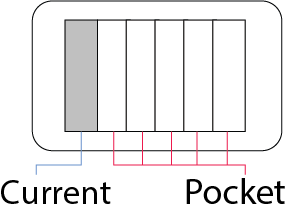
\includegraphics[height=4cm]{images/agent.png}
	\caption{\em Agente de población de MA.}
	\label{fig:agent}
\end{figure}

Los agentes que se usarán en el MA están compuestos por 6 soluciones, 1 \textit{Current} y 5 \textit{Pockets}, es decir, cada agente trabajará con una solución que irá evolucionando y tendrá 5 espacios de memoria reservado para guardar las mejores soluciones encontradas (ver figura \ref{fig:agent}).

\begin{equation*} 
    \begin{split} 
        Agente_i = \{Current, Pockets_{1{\times}5}\}
    \end{split} 
\end{equation*}


\subsubsection{Población}
\label{diseno:poblacion}
La estructura de la población de este método está compuesta por 13 agentes, dispuestos en un árbol ternario en 3 niveles con disposición jerárquica. A medida que se desciende en los niveles, las soluciones son peores, por lo tanto la mejor solución está en la raíz superior del árbol.
Este árbol está dispuesto en subpoblaciones, cada subpoblación contempla dos niveles del árbol, en el nivel superior está el agente líder y en el inferior sus 3 nodos hijos que corresponden a los agentes de apoyo. Cabe notar que los agentes ubicados en el segundo nivel del árbol general son líderes de las subpoblaciones inferiores y agentes de apoyo de la subpoblación superior.

\begin{figure}[tp]
	\centering
	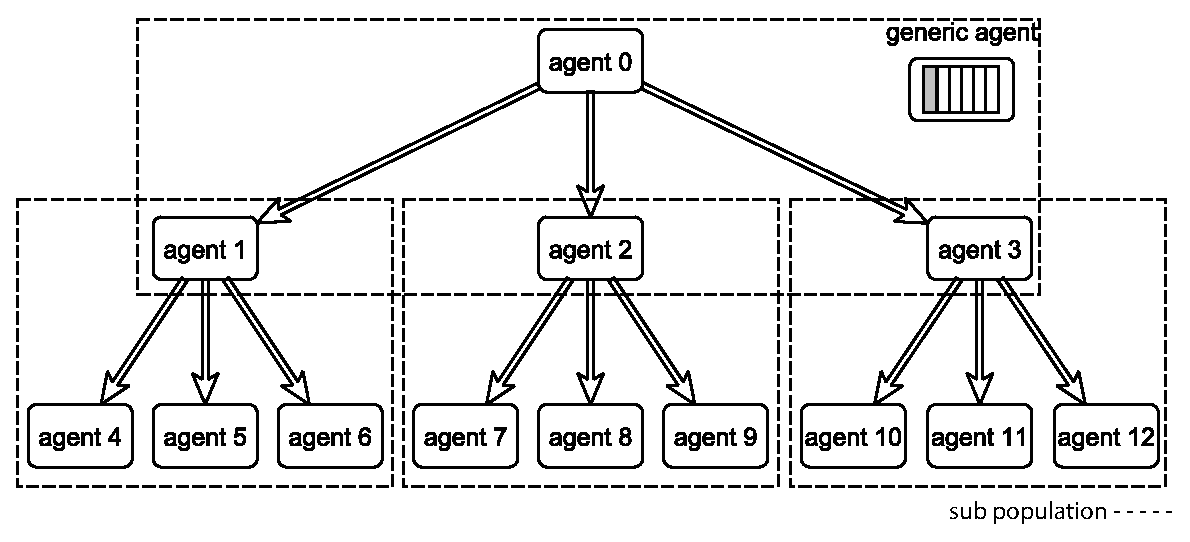
\includegraphics[height=6cm]{images/popStructure.eps}
	\caption{\em Estructura poblacional}
	\label{fig:ternary-pop}
\end{figure}

Tal como se puede ver en la figura \ref{fig:ternary-pop}, existen 4 subpoblaciones que están delimitadas por líneas segmentadas.

\begin{equation*} 
    \begin{split}
        Agente_{n} \text{ es lider de } SubPop_i \Longleftrightarrow n = i ~/~ &i = 0,1,2,3\\
            &n=0,1,\dots,12 \\
        \\    
        Agente_{n} \text{ es soporte de } SubPop_i \Longleftrightarrow n = 3i+j ~/~ &j = 1,2,3\\
        &i=0,1,2,3\\
        &n=0,\dots,12\\
    \end{split} 
\end{equation*}
\\[15pt]


Cada subpoblación tiene dos métodos importantes asociados:
\begin{itemize}
	\item \textbf{Actualización de pockets:} Todos los agentes deben evaluar si guardan la solución \textit{Current} en sus \textit{Pockets}. Esta acción tiene asociada reglas que aplican funciones como $d(A,B)$ que entrega \textit{Verdadero} si las soluciones A y B son diversas y $Energia(A)$ que entrega la energía potencial de la solución A. Con lo mencionado anteriormente, las reglas para realizar una inserción de una solución $S$ en los \textit{Pockets} de un $Agente_i$ son:
        \begin{enumerate}
            \item ($Agente_i$ no está completo) $\wedge$ ($d(S,Pocket^i_j))\geq
            10$), $\forall j$.
             \item ($Agente_i$ no está completo) $\wedge$
            (${\exists}j/d(S,Pocket^{i}_j){<}10$) $\wedge$
            ($Energia(S){<}Energia(Pocket^{i}_{mejor})$). Luego $S$ reemplazará a
            $Pocket^{i}_j$ / $d(S,Pocket^{i}_j))$ es mínima, $\forall j$.
             \item ($Agente_i$ está completo) $\wedge$ ($Energia(S) <
            Energia(Pocket^{i}_{mejor})$).Luego $S$ reemplazará a $Pocket^{i}_j$ /
            $d(S,Pocket^{i}_j))$ es mínima, $\forall j$.
            \item ($Agente_i$ está completo) $\wedge$ ($d(S,Pocket^{i}_j) \geq 10,
            \forall j$) $\wedge$ ($Energia(S) < Energia(Pocket^{i}_{peor})$). Luego $S$
            reemplzará a $Pocket^{i}_{peor}$.
        \end{enumerate}
	\item \textbf{Propagación de pockets:} después de la etapa anterior, el $Pocket_{mejor}$ de los agentes de apoyo es comparado con el $Pocket_{mejor}$ del agente líder de la subpoblación, si la solución del agente de apoyo es mejor que la del líder, se intercambian los pockets.
\end{itemize}

El método \textit{propagación de pockets} se aplica primero en las subpoblaciones inferiores y luego en la subpoblación superior, no al revés.

\subsection{Operadores del algoritmo mem\'etico}
A continuación se muestran los algoritmos de los operadores meméticos a ser implementados.

\subsubsection{Población inicial}

El algoritmo de población inicial se basa en la estructura jerárquica que se puede visualizar en la figura \ref{fig:ternary-pop}. Recibe como entrada la secuencia de aminoácidos que será usada en la predicción y entrega una población con 13 agentes con sus \textit{Currents} inicializados. 

Para ello, cada solución \textit{Current} se crea usando la información almacenada en la APL mediante el llamado a la función $obtenerAngulosDesdeAPL()$ (línea 7, Algoritmo \ref{alg:memetico-initpop}), esta función necesita como entrada el identificador del residuo y la estructura secundaria en la que se encuentra para escoger la APL correspondiente de la que se obtendrán los ángulos $\phi,\psi$. También usa la función $obtenerAngulosChi()$ (línea 9, Algoritmo \ref{alg:memetico-initpop}) para inicializar los valores de los ángulos de la cadena lateral, estos son provistos por la biblioteca Dunbrack (\citealp{dunbrack}) . Una vez que todos los residuos de la solución están completos, se calcula la energía de la solución (línea 12, Algoritmo \ref{alg:memetico-initpop}). Finalmente, se guarda la solución en el Current, este proceso se repite por cada agente de la población.
\\[25pt]
\begin{algorithm}[H]
	\begin{algorithmic}[1]
		\REQUIRE $secuencia$: secuencia de residuos
		\ENSURE $pop$: población de agentes
		\STATE $pop \leftarrow \textbf{popVacia}()$
		\FOR {$i=0:12$}
		    \STATE $pop[i] \leftarrow \textbf{agenteVacio}()$
			\STATE $sol \leftarrow \textbf{solVacia}()$
			\FOR {\textbf{each} residuo \textbf{in} $secuencia$}
				%\STATE $resid \leftarrow \textbf{obtenerAminoNumID}(residuo)$
				%\STATE $secundid \leftarrow \textbf{obtenerEstructuraSecundariaID}(residuo, secuencia)$
				\STATE \COMMENT ángulos $\phi$ y $\psi$ de la cadena principal
				\STATE $\phi,\psi \leftarrow \textbf{obtenerAngulosDesdeAPL}(sol, residuo, estruc)$
				%\STATE $\phi' \leftarrow \phi + random(-1,1)$
				%\STATE $\psi' \leftarrow \psi + random(-1,1)$
				\STATE \COMMENT ángulos $\chi$  de la cadena lateral
				\STATE $\chi_{angulos} \gets \textbf{obtenerAngulosChi}(residuo)$
				\STATE $sol.residuo[j] \leftarrow \phi,\psi,\chi_{angulos}$
			\ENDFOR
			\STATE $sol.energia \gets \textbf{calcularEnergia}(sol) $
			\STATE $pop[i].current \leftarrow sol$
		\ENDFOR
		\RETURN $pop$
	\end{algorithmic}
	\caption{Algoritmo Población Inicial}
	\label{alg:memetico-initpop}
\end{algorithm}

\subsubsection{Cruzamiento}
El algoritmo de cruzamiento tiene como fin otorgar la característica evolutiva al algorítmo memético, ya que mediante la reproducción se puede conservar características de las mejores soluciones a la vez que se diversifica la población, con la incorporación de las soluciones descendientes.

Respecto al funcionamiento, requiere dos soluciones A y B, que serán las soluciones que se cruzarán (Entrada de Algoritmo \ref{alg:memetico-cruzamiento}). Para generar la nueva solución, se crea una solución vacía y cada uno de sus residuos serán tomados del padre A o del padre B, para esta decisión se utiliza la función \textit{seleccionarDesdePadreA()} (línea 4, Algoritmo \ref{alg:memetico-cruzamiento}), si es verdadero se guardará la información del residuo del padre A en la nueva solución, de lo contrario, se tomará la información del residuo del padre B.
\\[25pt]
\begin{algorithm}[H]
	\begin{algorithmic}[1]
		\REQUIRE $sol_{A}$ y $sol_{B}$: soluciones a ser cruzadas
		\ENSURE \textit{descendiente}: nueva solución
		\STATE \textit{descendiente} $\leftarrow solVacia()$
		\FOR{$i=1:largoSecuencia$}
			\IF{$\textbf{hacerCruzamiento}()$}
    			\IF{$\textbf{seleccionarDesdePadreA}()$}
    				\STATE \textit{descendiente}.\textit{residuo}[i] $\gets sol_{A}.residuo[i]$
    			\ELSE
    				\STATE \textit{descendiente}.\textit{residuo}[i] $\gets sol_{B}.residuo[i]$
    			\ENDIF
			\ENDIF
		\ENDFOR
		\STATE \textit{descendiente.energia} $\gets \textbf{calcularEnergia}(descendiente)$
		\RETURN \textit{descendiente}
	\end{algorithmic}
	\caption{Algoritmo de Cruzamiento}
	\label{alg:memetico-cruzamiento}
\end{algorithm}

\subsubsection{Búsqueda local: \textit{Simulated annealing} con saltos de búsqueda}

Anteriormente se explicó la diferencia entre un individuo y un agente, se recalcó que un agente es un ente activo, esta actividad se ve reflejada en la capacidad de mejorar a lo largo del tiempo de manera conducida, para ello los agentes hacen uso de la búsqueda local que usa información característica del problema. En este trabajo se hace una adaptación del algoritmo de \textit{Enfriamiento Simulado (Simulated Annealing SA, \citealp{Kirkpatrick1983})} que implica la posibilidad de cambiar el punto de origen de la búsqueda.

\begin{figure}[tp]
	\centering
	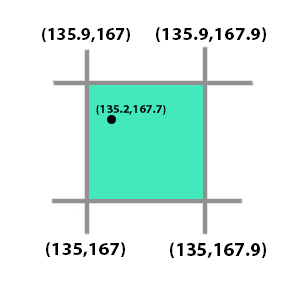
\includegraphics[scale=.7]{images/ls-range.jpg}
	\caption{\em Ejemplo de rango máximo de alcance del algoritmo de búsqueda local}
	\label{fig:ls-range}
\end{figure}

El algoritmo \ref{alg:localsearch} propone realizar una búsqueda local en la vecindad de los ángulos de cada uno de los residuos de la solución. En primera instancia se evalúa si se mantendrá el punto de origen, si se decide cambiar, la nueva coordenada deberá estar dentro del radio de búsqueda y será escogida usando la función $obtenerAngulosDesdeAPL()$. Luego, se procede a buscar dentro de la vecindad de la coordenada, la función \textit{escogerValorVecino()} buscará ángulos vecinos pero sin salir de la celda de la coordenada. Por ejemplo, si se tiene la coordenada $(135.2,167.7)$, se buscarán ángulos que no salgan de la celda delimitada por $(135.0,167.0)$, $(135.9,167.0)$, $(135.0,167.9)$, $(135.9,167.9)$ tal como se observa en la figura \ref{fig:ls-range}, la vecindad es la zona de color más claro. 
La cantidad de veces que se busca en la vecindad responde a la fórmula \ref{eq:sa-temperature}.
\begin{equation}
    \label{eq:sa-temperature}
    T(t)=T_{\text{inicial}}{\times}\alpha^t
\end{equation}
En donde $T$ es la función de temperatura del SA, $T_{\text{inicial}}$ es la temperatura inicial, $\alpha$ es el factor de enfriamiento y $t$ es el tiempo.

La probabilidad con la que es aceptada una solución es calculada según la ecuación \ref{eq:sa-prob}.

\begin{equation}
    \label{eq:sa-prob}
    P(energia_{mejor},energia_{sol},t) =
    \left\{
        \begin{array}{ll}
            V, & energia_{sol} < energia_{mejor} \\
            V, & exp(\frac{ energia_{mejor}-energia_{sol}}{T(t)}) > random(0,1) \\
            F, & exp(\frac{ energia_{mejor}-energia_{sol}}{T(t)}) \leq random(0,1)
            
        \end{array}
    \right.
\end{equation}
\\[25pt]

\begin{algorithm}[H]
    \begin{algorithmic}[1]
        \REQUIRE $sol$: solución, $salto$: salto máximo permitido 
        \ENSURE $sol$: solución final después de la búsqueda local
        \FOR {\textbf{each} residuo}
            \IF{$\textbf{hacerMejora()}$}
                \IF{$\textbf{cambiarCelda}()$} \label{line:changeAngleCell}
                    \STATE $sol \leftarrow \textbf{obtenerAngulosDesdeAPL}(sol,residuo,estruc,salto)$ \label{line:getAPL}
                    %\STATE $\phi' \leftarrow \phi + random(-1,1)$
                    %\STATE $\psi' \leftarrow \psi + random(-1,1)$
                \ENDIF
                \FOR{\textbf{each} $angulo (\phi,\psi)$ \textbf{in} $sol.residuo[i]$}
                    %\STATE $E_{anterior} \gets sol.energia$
                    %\STATE $energia_{aux} \gets energia_{anterior}$
                    \STATE $t = 0$
                    \REPEAT \label{line:iniSA}
                        %\STATE $sol_{respaldo} \gets sol$
                        \STATE $nuevaSol \gets \textbf{solVecina}(sol.residuo[i], angulo)$
                        \STATE $nuevaSol.energia \gets \textbf{calcularEnergia}(nuevaSol)$
                        \IF{$\textbf{P}(sol.energia,nuevaSol.energia,t)$}
                            \STATE $sol \gets nuevaSol$
                            %\STATE $sol.energia \gets energia_{aux}$
                    %    \ELSE
                    %        \STATE $sol \gets sol_{respaldo}$
                        \ENDIF
                        \STATE $t++$ \COMMENT aumenta la temperatura
                    \UNTIL{$\textbf{T}(t) < 0.1$} \label{line:endSA}
                    %\STATE $sol.energia \gets energia_{aux}$
                \ENDFOR
            \ENDIF
        \ENDFOR
    \RETURN $sol$
    \end{algorithmic}
    \caption{Algoritmo de Búsqueda Local}
    \label{alg:localsearch}
\end{algorithm}


\subsubsection{Mutación}
Con el fin de mantener la diversidad dentro de la población y aumentar la probabilidad de escapar de mínimos locales, se usa el algoritmo \ref{alg:memetico-mutation}. Esto se logra mediante la alteración de los ángulos de la cadena principal. Esta alteración consiste en la adición de un valor entre un intervalo a los ángulos $\phi$ y $\psi$ del residuo que se desea mutar. Cabe mencionar que la aplicación del operador de mutación está sujeto a la probabilidad de mutación ingresada como entrada.
\\[25pt]
\begin{algorithm}[H]
	\begin{algorithmic}[1]
		\REQUIRE$sol$: solución a ser mutada, \\ \hspace{1.2cm} $rango_{mutacion}$: valor que será sumado o restado al ángulo mutado.
		\ENSURE $sol$: solución mutada
		\FOR{$i=1:largoSecuencia$}
    		\IF{$\textbf{siHacerMutacion}()$}
    		    \STATE $sol.residuo[i] \gets sol.residuo[i] + random(-rango_{mutacion}, rango_{mutacion})$
    		\ENDIF
		\ENDFOR
		\STATE $sol.energia \gets \textbf{calcularEnergia}(sol)$
		\RETURN $sol$
	\end{algorithmic}
	\caption{Algoritmo de Mutación}
	\label{alg:memetico-mutation}
\end{algorithm}

\subsubsection{Diversidad}
El operador de diversidad responde si son diversas dos soluciones. Para ello, se basa en la suma de las distancias entre los ángulos de las dos soluciones. Estas distancias son calculadas haciendo uso de la lógica de los mapas de Ramachandran. Los ángulos dihédricos ($\phi$ y $\psi$) toman valores que van de -180$^\circ$ a 180$^\circ$ con la particularidad que -180$^\circ$ es equivalente que 180$^\circ$, por lo tanto, los bordes de los mapas de ramachandran son continuaciones de sus bordes opuestos.

Sea $A$ y $B$ dos soluciones, $D$ la diferencia mínima que debe existir para que dos soluciones sean diferentes, y $D_{A,B}$ la distancia entre $A$ y $B$, y $n$ el largo de la secuencia, la función de diversidad $d$ se define como:

\begin{equation}
    D_{A,B} = \frac{\sum_{i=1}^{n}min(|\Delta(\phi_i,\psi_i)_{A,B}|,360-(|(\phi_i,\psi_i)_{A}|+|(\phi_i,\psi_i)_{B}|))}{n}
\end{equation}

\begin{equation}
    \label{eq:diversity}
    d(S,R) =
    \left\{
        \begin{array}{ll}
            V, & D <  D_{A,B}   \\
            F, & D \geq D_{A,B} \\
        \end{array}
    \right.
\end{equation}
\\[25pt]
\begin{algorithm}[H]
	\begin{algorithmic}[1]
		\REQUIRE $sol_{A}$ y $sol_{B}$: soluciones a ser comparadas. $largoSecuencia$: largo de la secuencia de residuos
		\ENSURE valor de verdad que responde a la compración de las soluciones
		\STATE $diferencia=0$
		\FOR{$i=1:largoSecuencia$}
			\STATE $\phi_{A},\psi_{A} \gets sol_{A}.residuo[i]$
			\STATE $\phi_{B},\psi_{B} \gets sol_{B}.residuo[i]$
			\STATE $diferencia = diferencia + \textbf{min}(|\phi_{A}-\phi_{B}|,360-(|\phi_{A}|+|\phi_{B}|))$
			\STATE $diferencia = diferencia + \textbf{min}(|\psi_{A}-\psi_{B}|,360-(|\psi_{A}|+|\psi_{B}|))$
		\ENDFOR
		\STATE $diferencia = diferencia/largoSecuencia$
		\IF {$diferencia > diversidad$}
		    \RETURN \TRUE
		\ELSE
		    \RETURN \FALSE
		\ENDIF
	\end{algorithmic}
	\caption{Algoritmo de Diversidad}
	\label{alg:memetico-diversidad}
\end{algorithm}

\subsubsection{Actualización de la población}
Tal como se explicó en la sección \ref{diseno:poblacion}, la actualización de la población tiene como función guardar las mejores soluciones y propagar los \textit{pockets} a través de las subpoblaciones de manera ascendente, de forma que, a medida que se sube por el árbol ternario, se encuentren las mejores soluciones.
\\[25pt] 
\begin{algorithm}[H]
	\begin{algorithmic}[1]
		\REQUIRE $pop$: población de agentes
		\ENSURE $pop$: población de agentes ordenadas según estructura jerárquica

		\STATE \COMMENT Primer paso de actualización, guardar currents en pockets
		\FOR{$i=0:12$}
			\STATE $\textbf{reemplazarPeorPocket}(pop[i],pop[i].current)$
		\ENDFOR
		\STATE
		\STATE \COMMENT Segundo paso, propagar mejores pockets en las subpoblaciones inferiores
		\FOR{$i=1:3$}
			\STATE $x_{agente},y_{pocket} \gets \textbf{escogerMejorPocket}(pop[3i+1],pop[3i+2],pop[3i+3])$
			\IF{$pop[x_{agente}].pocket[y_{pocket}] < pop[i].pocket[0].energia$}
				\STATE $\textbf{intercambiarPockets}( pop[i].pocket[0], pop[x_{agente}].pocket[y_{pocket}])$
			\ENDIF
		\ENDFOR
		\STATE
		\STATE \COMMENT Tercer paso, propagar mejor pocket de la subpoblación superior
		\STATE $x_{agente},y_{pocket} \gets \textbf{escogerMejorPocket}(pop[1],pop[2],pop[3])$
		\IF{$pop[x_{agente}].pocket[y_{pocket}] < pop[0].pocket[0].energia$}
			\STATE $\textbf{intercambiarPockets}( pop[0].pocket[0], pop[x_{agente}].pocket[y_{pocket}])$
		\ENDIF
		
		\RETURN $pop$
	\end{algorithmic}
	\caption{Algoritmo de Actualización de la población}
	\label{alg:memetico-updatepop}
\end{algorithm}

\subsubsection{Reinicio}
El algoritmo de reinicio tiene como finalidad hacer escapar de la convergencia al algoritmo memético, reinicializando los \textit{currents} usando el operador APL y eliminando los 4 peores \textit{pockets} de todos los Agentes. Además, el algoritmo memético final incorpora un control de reinicio variable, es decir, toma en consideración la cantidad de generaciones que se necesitaron para converger, dicho tiempo lo considera como nueva cantidad máxima de generaciones sin mejora para realizar el próximo reinicio.
\\[25pt]
\begin{algorithm}[H]
	\begin{algorithmic}[1]
		\REQUIRE $pop$: población de agentes
		\ENSURE $pop$: población de agentes reiniciada
		\FOR{$i=0:12$}
			\STATE $pop[i].current\gets \textbf{nuevaSolucionAleatoria}()$
			\STATE \COMMENT se conserva $pop[i].pocket[0]$
			\STATE $pop[i].pocket[1] \gets \textbf{solVacia}()$
			\STATE $pop[i].pocket[2] \gets \textbf{solVacia}()$
			\STATE $pop[i].pocket[3] \gets \textbf{solVacia}()$
			\STATE $pop[i].pocket[4] \gets \textbf{solVacia}()$
		\ENDFOR
		\RETURN $pop$
	\end{algorithmic}
	\caption{Algoritmo de Reinicio}
	\label{alg:memetico-restart}
\end{algorithm}

\section{Algoritmo memético final}
Tras las explicaciones de los algoritmos y operadores principales que se usarán en la implementación final, se procede a la adaptación del algoritmo memético general para obtener el algoritmo principal (ver algoritmo \ref{alg:memetico-final}) que da solución al problema 3-D PSP.

Este algoritmo memético contempla como entrada la cantidad máxima de tiempo de ejecución medida en segundos, el número máximo de generaciones sin mejora para reiniciar la población del memético, y la estructura primaria y secundaria de la proteína.

Siguiendo al algoritmo general, se comienza haciendo uso del algoritmo de poblado inicial. Una vez inicializado cada \textit{current} de los 13 agentes, se realiza la actualización de la población para empezar a guardar y propagar los pockets de los agentes. Luego, en cada generación se realizará el cruzamiento de la subpoblación superior, esto significa que los \textit{currents} de los Agentes de apoyo serán poblados con el resultado del cruzamiento entre la solución guardada en el \textit{pocket[0]} del $Agente_0$ y el \textit{pocket[0]} de los \textit{Agentes de apoyo} respectivamente. Para terminar la etapa de cruzamiento se realiza el mismo procedimiento pero con las 3 subpoblaciones inferiores. Posteriormente, se busca mejorar los \textit{currents} mediante la aplicación del algoritmo de búsqueda local que hará uso del radio de salto, este radio irá disminuyendo a medida que pasan las generaciones, cuando el radio de búsqueda sea menor a 1 significa que no se podrán realizar más saltos. Finalmente se aplica el operador de mutación y se evalúa si el algoritmo debe reiniciar la población, para detectar si se debe realizar el reinicio se usa la cantidad de generaciones que la población no ha presentado mejoras, si este valor llega al máximo valor permitido (que ingresa como parámetro de entrada al algoritmo), se reinicia la población.
\\[25pt]
\begin{algorithm}[H]
    \begin{algorithmic}[1]
        \REQUIRE $tiempo_{max}$: tiempo de ejecución del MA, $secuencia$: secuencia de aminoácidos
        \ENSURE $sol_{mejor}$: mejor solución encontrada
%        \STATE $tiempo_{inicial} \gets obtenerTiempoActual()$
        \STATE \textit{//generación de población inicial aleatoria}
        \STATE $pop \gets \textbf{pobInicial}(secuencia)$
        \STATE $pop \gets \textbf{actualizarPob}(pop)$
        \STATE $sol_{mejor} \gets pop[0].pocket[0]; gen \gets 0$
        \STATE $contador \gets 0$; $radio \gets 90$
        \REPEAT
            \STATE \textit{//Selección y cruzamiento}
            \FOR{\textbf{each} agente$_i$, $i=1:12$}
            \STATE $padre_1 =
pop[\lfloor(i-1)/3\rfloor].pocket[random(1:5)]$ \label{line:par1}
            \STATE $padre_2 = pop[i].pocket[random(1:5)]$; \label{line:par2}
        \STATE $pop[i].cur \gets
\textbf{crossover}(pop[\lfloor(i-1)/3\rfloor].pocket[padre_1], pop[i].pocket[padre_2])$
            \STATE $pop[i].cur \gets \textbf{crossover}(padre_1,padre_2)$
\label{line:crossover}
            \ENDFOR
            \STATE \textit{//Búsqueda local y mutación}
            \FOR{$i=1:12$}
                \STATE $pop[i].cur \gets
\textbf{busquedaLocalSA}(pop[i].cur,radio)$
                \STATE $pop[i].cur \gets \textbf{mutacion}(pop[i].cur)$
            \ENDFOR
            \STATE $radio = 0.85{\times}radio$
            \STATE $pop \gets \textbf{actualizarPob}(pop)$
\textit{//Control de reinicio}
            \IF{$sol_{mejor} >= pop[0].pocket[0]$}
                \STATE $contador++$
            \ELSE
                \STATE $contador \gets 0$
                \STATE $sol_{mejor} \gets pop[0].pocket[0]$
            \ENDIF
            \IF{$contador == genSinMejora$}
                \STATE $pop \gets \textbf{reiniciarPob}(pop)$
\label{line:restart}
                \STATE $radio \gets 90$; $contador \gets 0$
                \STATE $genSinMejora \gets (gen-ultimoReinicio)$
                \STATE $ultimoReinicio \gets gen$
            \ENDIF
            \STATE $gen \gets gen + 1$
        \UNTIL $tiempo_{max}$
        \RETURN $sol_{mejor}$
        \end{algorithmic}
        \caption{Algoritmo memético final}
		\label{alg:memetico-final}
\end{algorithm}

\chapter{Criterios de evaluación y experimentos}
\label{cap:criterios}

En el presente capítulo se aborda el plan de experimentación y criterios de evaluación que se aplican a los resultados en el capítulo \ref{cap:resultados}.

\section{Diseño de experimentos}

\subsection{Plan de Pruebas}
Debido a que la solución desarrollada es de naturaleza estocástica, se requiere ejecutar múltiples instancias para una misma proteína con el fin de evaluar el comportamiento general del algoritmo. Para ello se ha decidido correr 10 ejecuciones de 24 horas por cada proteína. Las proteínas y cantidad de residuos se pueden ver en la tabla \ref{table:lista-proteinas}. Además, con el fin de verificar la contribución de las APLs al MA se decidió realizar el mismo plan de pruebas pero sin incorporar esta información. Para ello, todas las secciones del MA que piden información a las APLs fueron reemplazadas por una función que devuelve un valor flotante aleatorio entre $-180^\circ$ y $180^\circ$.

\begin{table}[h]
	\centering
	\caption{Proteínas de prueba}
	\begin{tabular}{|c|c|}
		\hline
		\textbf{PDB ID } & \textbf{Cantidad de residuos} \\ \hline
		2EVQ 	& 12		\\		
		1DV0 	& 45		\\ 	
		1DEP 	& 15		\\  
		1E0Q 	& 17		\\ 	
		1K43 	& 14		\\ 
		1L2Y 	& 20		\\		\hline
	\end{tabular}
	\label{table:lista-proteinas}
\end{table}

Para la ejecución de instancias se usó 8 computadores idénticos modelo HP EliteDesk 800-G1-SFF cuyas características principales son:
\begin{itemize}
	\item CPU Intel Core i7 3.4Ghz de 8 núcleos físicos.
	\item 8Gb de RAM.
	\item Unidad de almacenamiento SSD de 120Gb.
\end{itemize}

Por lo tanto, los equipos en su totalidad pueden correr hasta 80 ejecuciones en paralelo. Como se tienen 6 proteínas de prueba y 10 ejecuciones de 24 horas por cada una, se obtienen 1440 horas de ejecución que al dividirlo por la cantidad de núcleos disponibles da un total de 22.5 horas continuas de ejecución.

\begin{equation}
	\frac{6\text{proteínas}{\times}10\text{ejecuciones}{\times}24\text{horas}}{80\text{núcleos}} = 22.5\text{horas}
\end{equation}

Esta cantidad de horas es la misma para el plan de pruebas que no considera las APLs en el MA. Por lo tanto, los experimentos que involucran estas 6 proteínas toman 2 días de ejecución.

También, solo con el fin de ver como se comporta el MA con proteínas más extensas, se decidió probar 9 proteínas (ver tabla \ref{table:prot-ext}) ejecutando una instancia del MA por cada una de ellas, cada instancia toma 72 horas. Para esta prueba se usó el recurso Bioserver disponible en el Departamento de Ingeniería Informática de la Universidad de Santiago, cuya configuración es:

\begin{itemize}
\item Procesador Intel Xeon E5-2609 (10M Caché, 2.40 GHz)
\item Memoria RAM DDR3 de 16GB
\end{itemize}


\begin{table}[h]
	\centering
	\caption{Proteínas extensas de prueba}
	\begin{tabular}{|c|c|}
		\hline
		\textbf{PDB ID} & \textbf{Cantidad de residuos} \\ \hline
		 2F4K & 35\\
         2JUC & 59\\
         2MR9 & 44\\
         2P5K & 64\\
         2P81 & 44\\
         3P7K & 45\\
         3V1A & 43\\
         2MQ8 & 112\\
         2MW1 & 119\\ \hline
	\end{tabular}
	\label{table:prot-ext}
\end{table}

\subsection{Herramientas utilizadas en la implementación}

\subsubsection{AmberTools 14}
\textit{AmberTools} es un conjunto de programas destinados para la simulación y análisis biomolecular (\citealp{amber14}). Cada aplicación de este paquete ha sido diseñado para que pueda trabajar con los demás. La mayoría de los componentes de AmberTools está distribuido bajo licencia \textit{GNU General Public License (GPL)}. Este paquete contiene un lenguaje de programación especial para realizar simulaciones conocido como \textit{\textbf{NAB (Nucleotic Acid Builder) Language}} permitiendo usar distintos campos de fuerza dependiendo del tipo de simulación. Debido a esta ventaja, se ha decido usar esta suite para construir la solución. 

\subsubsection{Lenguaje de programación NAB}
NAB fue originalmente diseñado como un lenguaje de modelación pequeño con el objetivo principal de construir modelos no helicoidales de ácidos nucléicos. Con el éxito del proyecto, se agregó a su implementación el campo de fuerza de Amber \textit{(Amber Force Field o AMBER14FF, \citealp{simmer})}. 

NAB provee soporte especializado en su lenguaje para el uso de macromoléculas y sus componentes, lo que da flexibilidad al programador y no limita los tipos de simulaciones, Este lenguaje tiene una sintaxis muy parecida a C, y al momento de la compilación es transformado a código C para luego ser compilado a binario. Además, este lenguaje de programación contiene bibliotecas que proveen de funciones ya programadas y listas para ser usadas, que van desde el cálculo de distancia molecular a funciones propias de la dinámica molecular.

\subsubsection{AMBER Force Field}
Este trabajo está basado en los avances de \cite{Dorn:2013}. Dicha investigación usa el campo de fuerza Amber en su versión \textit{AMBER99}. No obstante, según la documentación de AmberTools 14, para la simulación biomolecular de una secuencia de aminoácidos se recomienda usar la versión actualizada del campo de fuerza, que corresponde a \textit{AMBER14FF} (\citealp{simmer}).

La función de energía potencial de Amber se calcula según la siguiente fórmula:

\begin{equation}
\begin{split}
E_{total}=\sum_{bonds}\frac{1}{2}K_{b}(b-b_{0})^2 + \sum_{angles}\frac{1}{2}K_{\theta}(\theta-\theta_{0})^2 + \sum_{torsions}\frac{1}{2}K_{\eta}(1+\cos(\eta_{\omega}-\gamma)) \\
+ \sum_{j=1}^{N-1}\sum_{i=j+1}^{N-1}\left\{ \epsilon_{i,j}\left[ \left( \frac{R_{0ij}}{r_{ij}} \right)^{12}-2\left( \frac{R_{0ij}}{r_{ij}} \right)^{6} \right] + \frac{q_{i}q_{j}}{4\pi\epsilon_{0}r_{ij}} \right\}
\end{split}
\end{equation}
dónde:
\begin{itemize}
	\item \textit{Bonds}: representa la energía entre los átomos unidos por enlaces covalentes
	\item \textit{Angles}: representa la energía debido a la geometría de las órbitas del electrón envueltos en los enlaces covalente.
	\item \textit{Torsions}: representa la energía para girar un enlace debido el orden de los enlaces, a la presencia de enlaces vecinos o a pares solitarios de electrones.
	\item El último término corresponde la energía de los componentes no enlazados, que tal como se revisó en la ecuación \ref{eq:nonbonded}, corresponde a la energía electrostática y fuerzas o interacciones de \textit{van} der Waals.
\end{itemize}

\subsubsection{STRIDE}
STRIDE \textit{Structural Identification} (\citealp{stridepaper}) es un algoritmo de asignación de estructuras secundarias de la proteína. STRIDE es similar al algoritmo DSSP, usa los enlaces de hidrógeno como criterio de clasificación pero también agrega los potenciales de los ángulos diedros. Por lo tanto, el criterio de clasificación de STRIDE es más completo y ha reportado asignaciones más satisfactorias en comparación a DSSP (\citealp{zhang:2015}). Por lo que se ha optado por STRIDE para predecir la estructura secundaria de las proteínas en estudio.


\section{Criterios algorítmicos de evaluación }
El análisis algorítmico evalúa la efectividad y eficiencia del algoritmo implementado, de la cual se puede obtener información para realizar modificaciones y mejoras. Para ello se expone las curvas de convergencia y la parametrización usada.

\subsection{Tiempos de convergencia}
Los tiempos de convergencia indican cuan rápido el algoritmo converge a una solución, este indicador sirve especialemente para evaluar cada cuánto tiempo se deben hacer reinicios de la población y los posibles cambios en la parametrización del algoritmo.

\subsection{Parámetros}
Los parámetros usados en la implementación del algoritmo son los siguientes:
\begin{itemize}
	\item \textbf{MAX\_SECS}: cantidad máxima de tiempo de ejecución en segundos.
	\item \textbf{MAX\_GENS\_NOIMPROVE}: cantidad máxima de generaciones sin mejora.
	\item \textbf{LS\_PROB}: probabilidad de aplicar el operador búsqueda local. 
	\item \textbf{DIVERSITY}: valor considerado como diversidad.
	\item \textbf{CROSSOVER} probabilidad de seleccionar residuos el primer padre.
	\item \textbf{MUT\_ADJUSTMENT}: rango de mutación.
	\item \textbf{MUT\_PROB}: probabilidad de aplicar el operador de mutación.
	\item \textbf{JUMP\_PROB}: probabilidad de cambiar el punto de origen al hacer búsqueda local.
	\item \textbf{JUMP\_RADIUS}: radio máximo de salto al cambiar el punto de origen en la búsqueda local.
	\item \textbf{JUMP\_FACTOR}: factor que permite decrecer al radio de salto.
\end{itemize}

Finalmente, en este capítulo se presentan la duración y distribución de los experimentos, la batería de proteínas que se probarán y las aristas que serán evaluadas de las soluciones generadas por el algoritmo memético.

\section{Criterios biológicos de evaluación }

Desde un comienzo se ha comentado que el MA actúa en base a una función de minimización de energía que usa un operador de búsqueda local para alcanzar mejores soluciones. No obstante, la evaluación de las soluciones no puede ser solo desde ese punto de vista ya que el encontrar menores energías no implica que la solución sea la mejor. Esto se debe principalmente a las falencias que presentan los campos de fuerza existentes para simular el entorno atómico (\citealp{hornak:2006}). Es por ello que se evaluará su similitud tridimensional y de estructuras secundarias, y comportamiento estereoquímico.

\subsection{Análisis RMSD}
El RMSD (ecuación \ref{rmsd-eq}) es la medida promedio de la distancia entre átomos Carbono $\alpha$ ($C_{\alpha}$) en el espacio que se produce por la superposición de estructuras. La unidad de esta medida es en Ångströms.

\begin{equation}
RMSD(a,b) = \sqrt{\frac{1}{n}\sum_{i=1}^{n}||r_{ai} - r_{bi}||^2}
\label{rmsd-eq}
\end{equation}

Para este análisis se usará la herramienta PROFIT, en la superposición se descartan los tres primeros y últimos residuos, ya que las proteínas presentan vibraciones y puntos de alta flexibilidad en los extremos que de considerarse implicaría un cálculo impreciso lo que puede dar una noción errada en el cálculo de RMSD. 

\subsection{Análisis de estructura secundaria}
Este análisis toma las soluciones creadas por el algoritmo memético, evalúa las estructuras secundarias detectadas y las compara con los estados conformacionales de la proteína experimental. STRIDE será la herramienta encargada de la determinación.
Se considerarán las soluciones cuya energía sea la más baja y RMSD más bajo. Para el análisis visual se usará la herramienta PYMOL (\citealp{pymol}), ya que permite la visualización de las proteínas generadas en tres dimensiones además de dibujar las estructuras secundarias, también permite la superposición de estructuras con lo que se podrá apreciar la calidad de la solución predicha y la proteína experimental.

\subsection{Análisis Estereoquímico}
El análisis estereoquímico estudia las reacciones e interacciones producto de la disposición espacial de los átomos. Por ejemplo, en las predicciones de estructura de proteínas se debe tratar de minimizar los choques esteroquímicos, a medida que la solución presenta más choques, es más probable que no sea de buena calidad biológica. La herramienta PROCHECK (\citealp{procheck}) entrega mapas de Ramachandran con las áreas seguras o de baja probabilidad de choques estereoquímicos e indica la posición de los átomos de la solución evaluada en el mapa. 

\subsection{Comportamiento proteínas extensas}

Con el fin de tener una mejor visión sobre el comportamiento del algoritmo y sus posibles modificaciones, es que se realizará la prueba de RMSD y visual a un conjunto de 9 proteínas cuya extensión va desde los 35 a 119 residuos de aminoácidos.
\chapter{Resultados}
\label{cap:resultados}
En este capítulo se presentan los resultados obtenidos tras la ejecución del plan de pruebas propuesto en el capítulo anterior.

\section{Evalución algorítmica}

\subsection{Convergencia}
El algoritmo memético hace uso de un control de reinicio que se adapta según el tiempo que le toma en cada convergencia. Tras converger, guarda la cantidad de generaciones \textit{G} que le tomó estancarse y se reinicia la población según el algoritmo \ref{alg:memetico-restart}, luego el MA tiene G generaciones para poder encontrar una mejor solución antes de volver a reiniciar la población. A continuación, se exponen los gráficos de convergencia del algoritmo para cada una de las 6 proteínas probadas en este trabajo. Se puede apreciar la contribución de los reinicios de la población al resultado final que entrega el MA. Los gráficos expuestos corresponden a las ejecuciones que entregaron las energías más bajas para cada proteína.

\begin{figure}
\centering
\begin{tabular}{c c}
\\
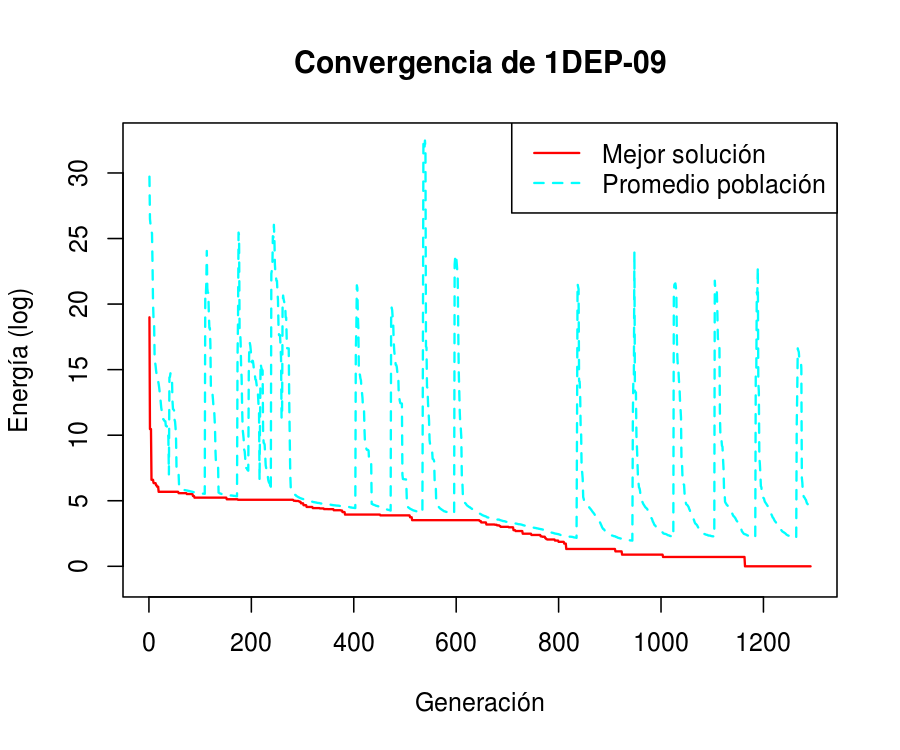
\includegraphics[height=6cm]{images/convergencia-1DEP-09.png} & 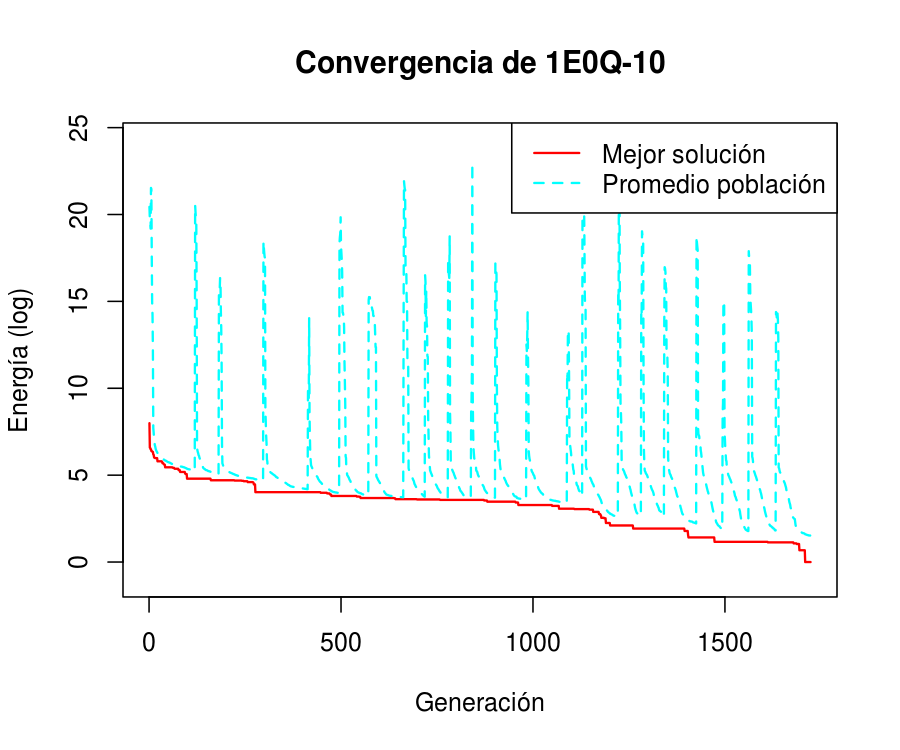
\includegraphics[height=6cm]{images/convergencia-1E0Q-10.png} \\
(a) & (b) \\
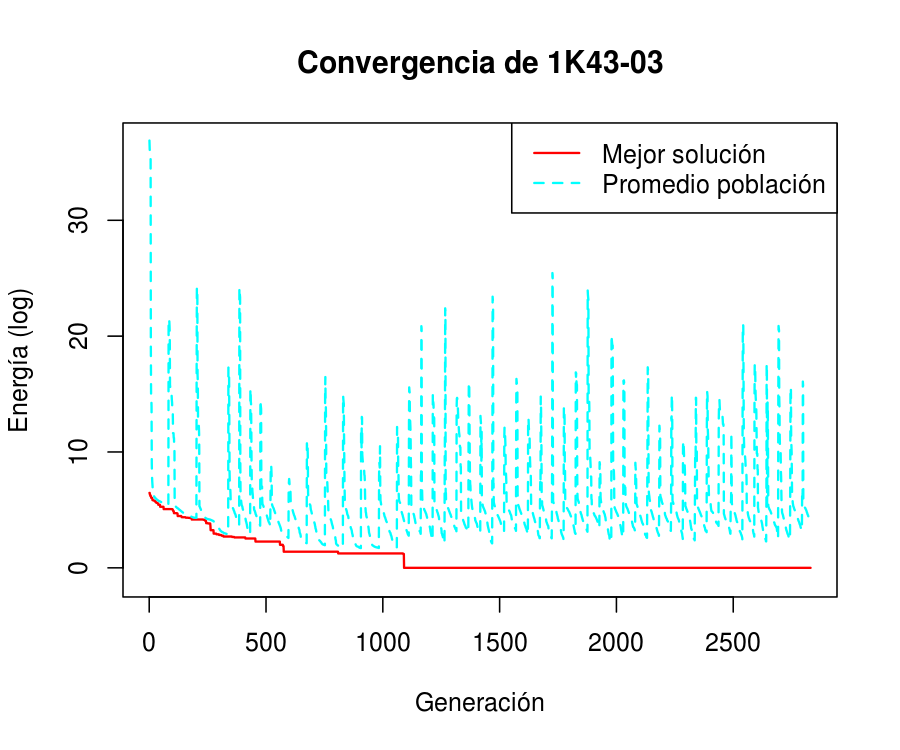
\includegraphics[height=6cm]{images/convergencia-1K43-03.png} & 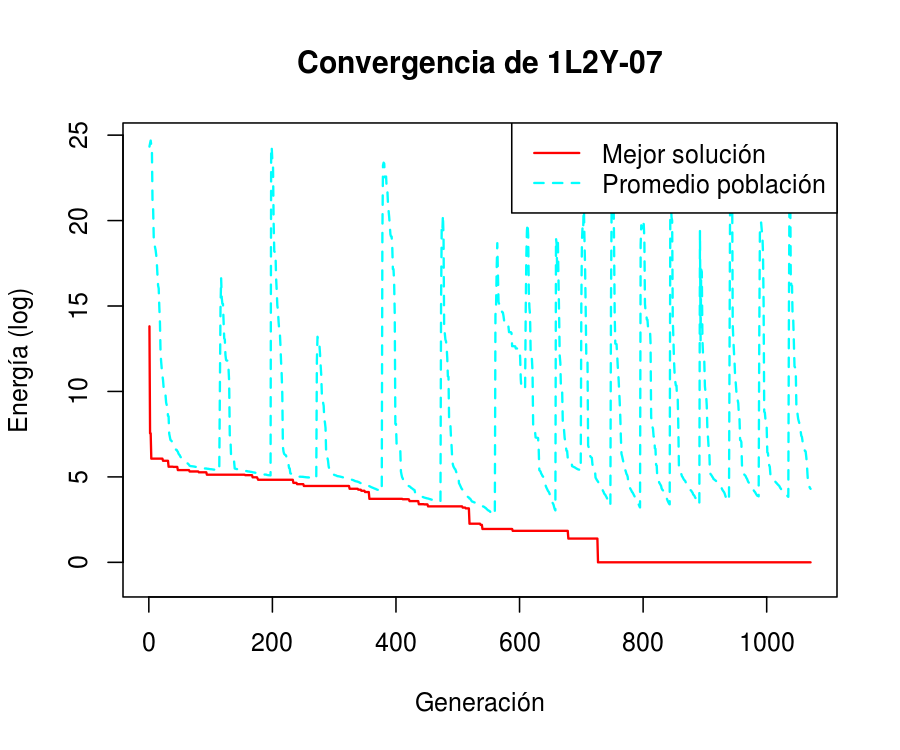
\includegraphics[height=6cm]{images/convergencia-1L2Y-07.png} \\
(c) & (d) \\
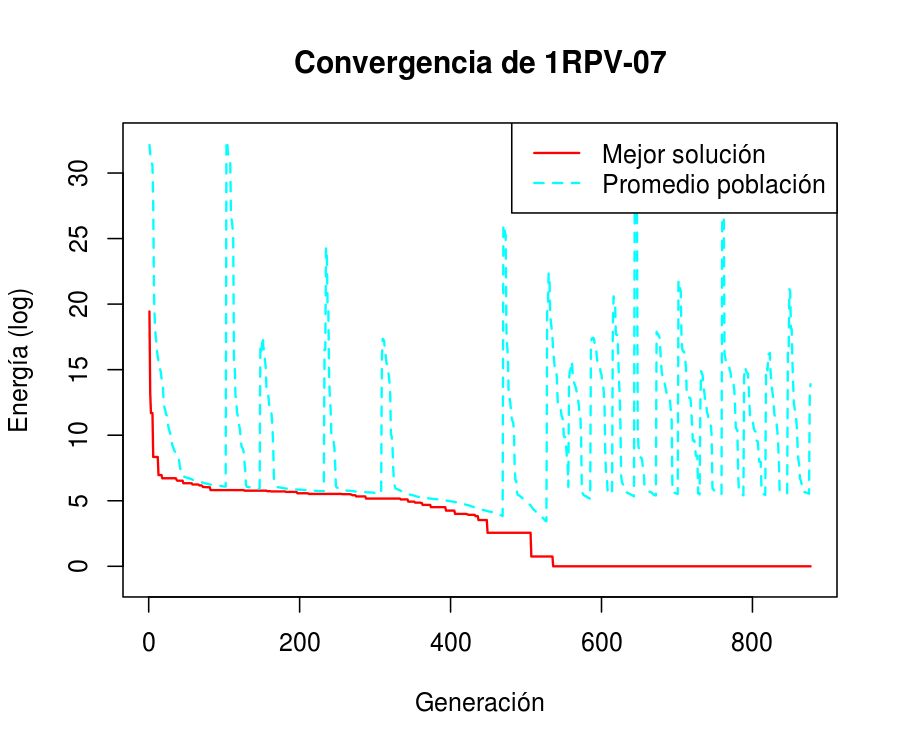
\includegraphics[height=6cm]{images/convergencia-1RPV-07.png} & 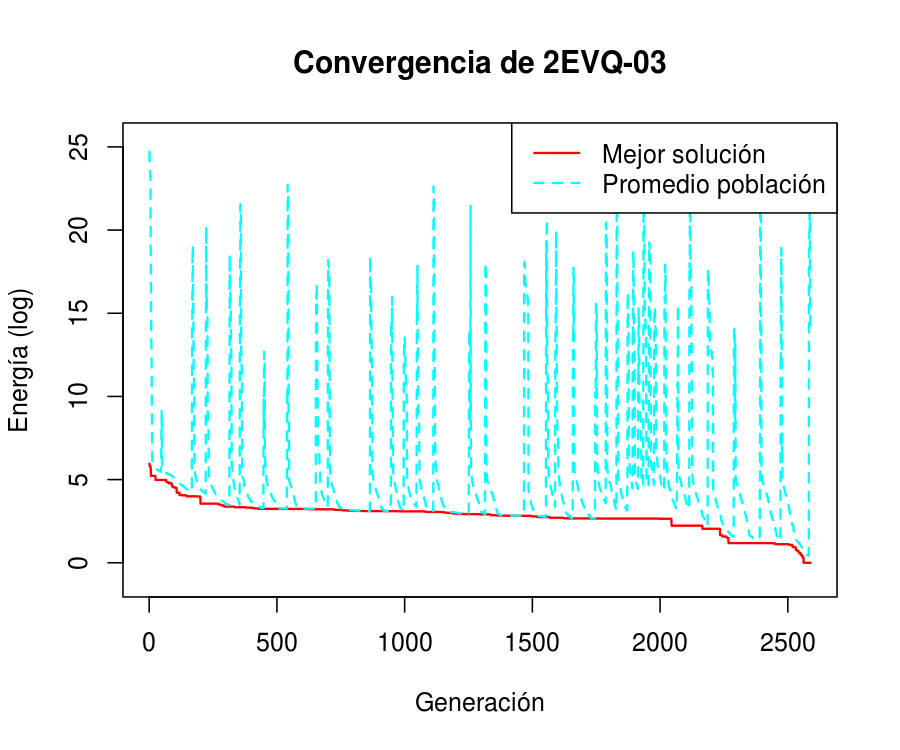
\includegraphics[height=6cm]{images/convergencia-2EVQ-03.png} \\
(e) & (f) \\

\end{tabular}
\caption[Curvas de convergencia]{Ejemplos de curvas de convergencia del algoritmo mem\'etico para las proteinas (a) 1DEP, (b) 1E0Q, (c) 1K43, (d) 1L2Y, (e) 1RPV y (f) 2EVQ}
\label{fig:convergencia}
\end{figure}

En la figura \ref{fig:convergencia} se puede observar la contribución del control de reinicio a la mejor solución al enfrentarse con la convergencia de la población de agentes. Por otra parte, existen casos con problemas de convergencia en sus últimas generaciones (gráfico (c) figura \ref{fig:convergencia}  de la generación 1000 en adelante), una forma de solucionar este problema podría ser mediante la implementación de un control de reinicio completo de la población (sin preservación de soluciones).


\subsection{Parámetros}
Los parámetros usados para la experimentación fueron establecidos tras pruebas de corta duración (1 a 3 horas) a medida que se realizaba la implementación del MA, haciendo uso delas proteínas 1K43 y 1L2Y, ya que estas presentas zonas de díficil predicción (hojas-$\beta$ y vueltas). No fue posible realizar una parametrización más rigurosa debido al tiempo del que se disponía para la construcción y implementación del MA. Los parámetros usados en las pruebas están presentes en la tabla \ref{table:lista-valores-parametros}.

\begin{table}[h]
	\centering
	\caption{Parámetros usados en las pruebas}
	\begin{tabular}{|l|r|}
		\hline
		Parámetro & Valor \\ \hline
		MAX\_SECS 	& 86400		\\		
		MAX\_GENS\_NOIMPROVE 	& 20		\\ 		
		LS\_PROB 	& 0.9		\\  	
		DIVERSITY 	& 10.0		\\ 		
		CROSSOVER 	& 0.4		\\ 		
		MUT\_ADJUSTMENT 	& 0.05		\\ 		
		MUT\_PROB 	& 0.5		\\		
		JUMP\_PROB 	& 0.3		\\		
		JUMP\_RADIUS 	& 90		\\		
		JUMP\_FACTOR 	& 0.85		\\	\hline	
	\end{tabular}
	\label{table:lista-valores-parametros}
\end{table}

\section{Calidad biológica de las soluciones}

\subsection{Contribución APL}

La tabla \ref{table:results-apl-noapl} muestra el resumen de los resultados generados por el Algoritmo Memético que hace uso de la APL en contraste cuando obtiene valores aleatorios para los ángulos de torsión.

\begin{table}[h]
	\centering
	\caption[Análisis comparativo de resultados de APL y Sin APL]{Análisis comparativo de resultados obtenidos de MA con APL y sin APL. Energía medida en $Kcal/mol$ y RMSD medido en $\AA$}
\begin{tabularx}{\textwidth}{|l|r|r|r|r|r|r|} \hline
{PDB} & \multicolumn{2}{c|}{APL} & \multicolumn{2}{c|}{Sin APL} & \multicolumn{2}{c|}{\textit{p-value}}\\ \cline{2-7}
 {ID} & \multicolumn{1}{c|}{Energía} & \multicolumn{1}{c|}{RMSD} & \multicolumn{1}{c|}{Energía} & \multicolumn{1}{c|}{RMSD} & \multicolumn{1}{c|}{Energía} & \multicolumn{1}{c|}{RMSD} \\ \hline
 {2EVQ} & -94.2 (-70.2) & 3.58 (2.87) & -92.6 (-40.8) & 3.76 (2.76) & $8.398^{-2}$ & $4.922^{-1}$   \\
 {1K43} & -558.6 (-515.2) & 2.50 (2.71) & -447.8 (-405.0) & 5.05 (4.77 ) & $\mathbf{1.953^{-3}}$ & $\mathbf{1.953^{-3}}$\\
 {1DEP} & -304.2 (-272.7) & 1.43 (1.03) & -377.3 (-239.2)  & 4.12 (4.28) & $3.750^{-1}$ & $\mathbf{5.889^{-3}}$\\
 {1E0Q} & -280.9 (-236.7) & 7.08 (4.77) & -141.2 (-49.4) & 5.04 (5.41 ) & $\mathbf{1.953^{-3}}$ & $4.922^{-1}$  \\
 {1RPV} & -1027.9 (-937.3) & 2.15 (1.88) & -1075.1 (-947.3) & 5.66 (5.66 ) & $5.566^{-1}$ & $\mathbf{1.953^{-3}}$  \\
 {1L2Y} & -261.9 (-225.7) & 5.43 (4.04) & -187.4 (-23.8) & 5.01 (5.39 ) & $\mathbf{1.953^{-3}}$ & $\mathbf{9.766^{-3}}$ \\ \hline
\end{tabularx}
\label{table:results-apl-noapl}
\end{table}

Para validar estadísticamente estos resultados, la columna \textit{p-value} de la tabla \ref{table:results-apl-noapl} muestra los valores arrojados por el test de Wilcoxon que se utiliza para comparar dos mediciones de rangos y determinar que la diferencia no se deba al azar. Dado dichos resultados, se comprueba estadísticamente que la contribución de la APL es estadísticamente significativa.


\subsection{Análisis RMSD}

La tabla \ref{table:results-summary} muestra el resumen de las 10 ejecuciones del MA sobre cada secuencia. El MA es capaz de alcanzar bajos valores de energía mientras a la vez alcanza buenas soluciones en términos de RMSD. Las imágenes de la figura \ref{fig:rmsd-proteinas} muestran las comparaciones realizadas mediante la alineación espacial de las soluciones con mejor RMSD, mejor energía y la estructura experimental correspondiente.

\begin{table}[h]
\small
\centering
\caption[Resumen de resultados]{Resumen de resultados usando APL, tomando las mejores soluciones obtenidas por el MA desde el punto de vista RMSD y energía.}
\scalebox{1}{
\begin{tabular}{|c|r|r|c|c|r|r|} \hline
\multirow{2}{*}{PDB} & \multicolumn{1}{c|}{Menor} & \multicolumn{1}{c|}{Promedio} & \multicolumn{1}{c|}{RMSD (\AA)} & \multirow{1}{*}{Menor}& \multirow{1}{*}{Promedio} & \multicolumn{1}{c|}{Promedio}\\

\multirow{2}{*}{ID} & \multicolumn{1}{c|}{Energía} & \multicolumn{1}{c|}{Energía} & \multicolumn{1}{|c|}{Menor} & \multirow{1}{*}{RMSD (\AA)}& \multirow{1}{*}{RMSD (\AA)} & \multicolumn{1}{c|}{Número de}\\

 & \multicolumn{1}{c|}{($\text{Kcal}/\text{mol}^{-1}$)} & \multicolumn{1}{c|}{($\text{Kcal}/\text{mol}^{-1}$)} & \multicolumn{1}{c}{Energía} & \multicolumn{1}{|c|}{} & \multicolumn{1}{|c|}{} & \multicolumn{1}{c|}{Generaciones}\\
\hline
{2EVQ} & -94.21  & -70.24 ($\pm$14.69)   & 3.58   & 1.35  & 2.87 ($\pm$0.84)  & 3760.3\\\hline
{1K43} & -558.56  & -515.16 ($\pm$36.40)   & 2.50   & 1.27  & 2.71 ($\pm$0.83)  & 2536.8\\\hline
{1DEP} & -304.16  & -272.69 ($\pm$24.42)   & 1.43   & 0.39  & 1.03 ($\pm$0.44)  & 1414.3\\\hline
{1E0Q} & -280.86  & -236.72 ($\pm$32.21)   & 7.08   & 2.21  & 4.77 ($\pm$2.1)  &  1389.8\\\hline
{1RPV} & -1027.95  & -937.26 ($\pm$76.88)   & 2.15   & 0.97  & 1.88 ($\pm$0.46)  & 834.5\\\hline
{1L2Y} & -261.90  & -225.65 ($\pm$32.36)   & 5.43   & 2.26  & 4.04 ($\pm$1.10)  & 1027.1\\\hline
\end{tabular}}\label{table:results-summary}
\end{table}



\begin{figure}
\centering
\begin{tabular}{c c}
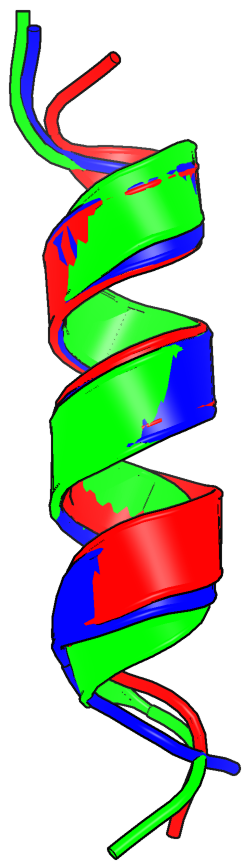
\includegraphics[height=5.2cm]{images/rmsd-1DEP.png} & 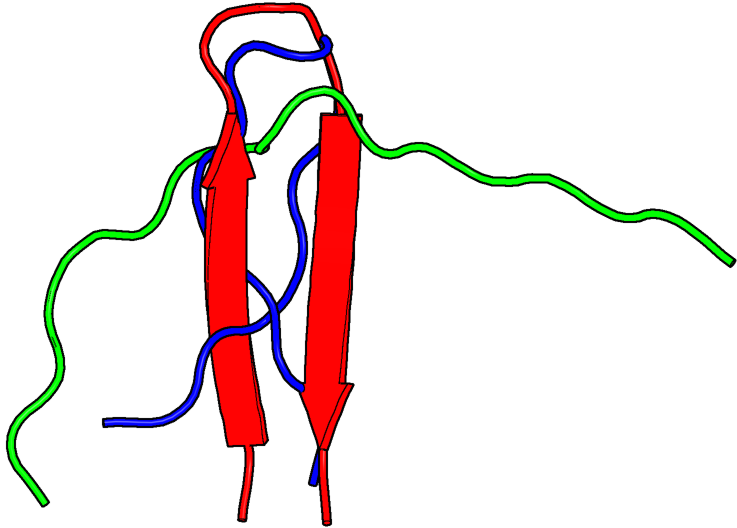
\includegraphics[height=5.2cm]{images/rmsd-1E0Q.png} \\
(a) & (b) \\ \\
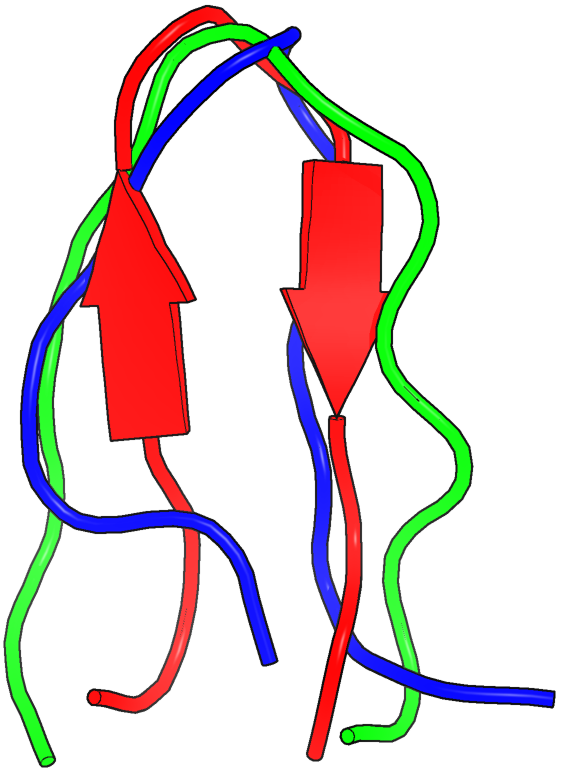
\includegraphics[height=5.2cm]{images/rmsd-1K43.png} & 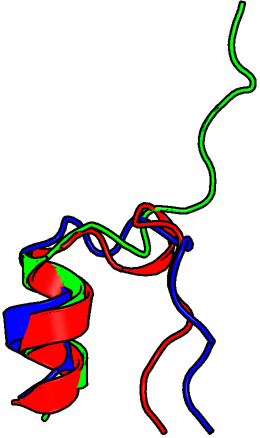
\includegraphics[height=5.2cm]{images/rmsd-1L2Y.png} \\
(c) & (d) \\ \\
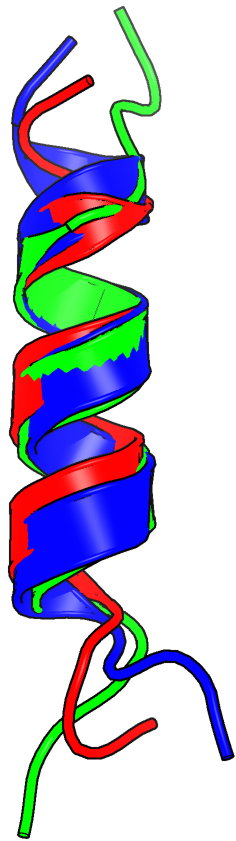
\includegraphics[height=5.2cm]{images/rmsd-1RPV.png} & 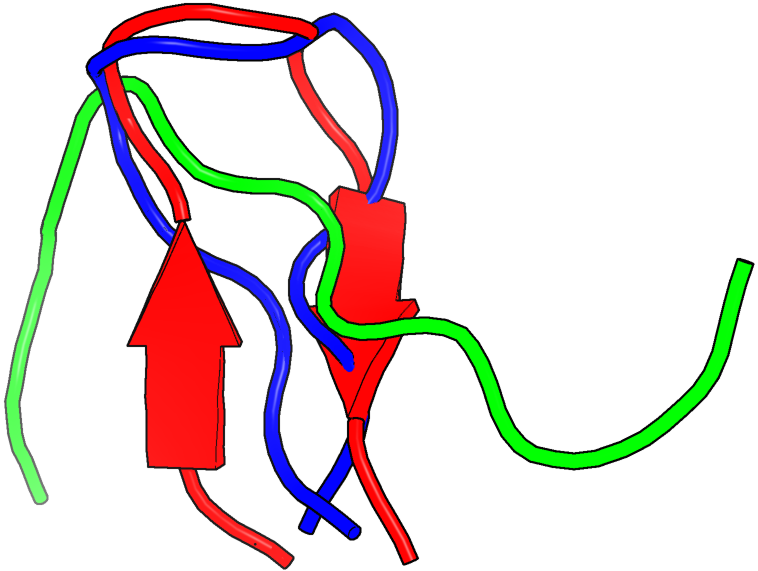
\includegraphics[height=5.2cm]{images/rmsd-2EVQ.png} \\
(e) & (f) \\

\end{tabular}
\caption[Alineación espacial de estructuras]{Resultados de alineación espacial para las proteínas (a) 1DEP, (b) 1E0Q, (c) 1K43, (d) 1L2Y, (e) 1RPV y (f) 2EVQ. Solución con mejor energía en color verde, mejor RMSD en azul y estrcutura experimental en rojo. Las estructuras fueron alineadas a partir de la superposición de sus $C_{\alpha}$ utilizando PyMol.}
\label{fig:rmsd-proteinas}
\end{figure}


Es importante recordar que el usar la energía como función de minimización \textbf{no garantiza que la mejor solución en términos de energía tendrá el mejor RMSD} cuando se compare con la proteína experimental. En la tabla \ref{table:results-summary} la mejor solución en términos de RMSD no corresponde a la solución que obtiene la energía más baja.

\subsection{Análisis de estructura secundaria}

La tabla \ref{table:stridess} compara las estructuras secundarias de las soluciones obtenidas por el algoritmo contra las proteínas experimentales. 

\begin{table}[H]
\centering
\caption[Resultados PROMOTIF]{Resultados de PROMOTIF para las estructuras experimentales (E) y soluciones con menor energía (P).}

\begin{tabular}{|l|r|r|r|r|}\hline
{PDB ID} & \% hojas-$\beta$ & \% hélices-$\alpha$ & \% hélices-$3^{10}$ & \% Otras\\\hline

2EVQ-E & 50 & 0 & 0 & 50\\
2EVQ-P & 0 & 0 & 0 & 100\\\hline

1K43-E & 43  & 0 & 0 & 57\\
1K43-P & 0 & 0 & 0 & 100\\\hline

1DEP-E & 0 & 80 & 0 & 20\\
1DEP-P & 0 & 54 & 13 & 33\\\hline

1E0Q-E & 71 & 0 & 0 & 29\\
1E0Q-P & 0 & 0 & 0 & 100\\\hline

1RPV-E & 0 & 65 & 0 & 35\\
1RPV-P & 0 & 59 & 0 & 41\\\hline

1L2Y-E & 0 & 35 & 20 & 45\\
1L2Y-P & 0 & 40 & 0 & 60\\\hline
\end{tabular}
\label{table:stridess}
\end{table}

Este análisis revela que la topología de las soluciones predichas y las experimentales son comparables a las estructuras experimentales. En general, el MA propuesto tiene problemas en la predicción de hojas-$\beta$ y áreas de curvatura (se puede apreciar en la tabla \ref{table:stridess} en las proteínas 2EVQ, 1k43 y 1E0Q), no así con la predicción de hélices (ver proteínas 1RPV, 1DEP y 1L2Y).  

\subsection{Análisis Estereoquímico}

La tabla \ref{table:procheck} resume numéricamente los valores del gráfico de Ramachandran para las proteínas experimentales y estructuras predichas.

\begin{table*}[!htb]
\centering
\caption{Valores de los gráficos de Ramachadran para las estructuras experimentales(E) y predichas(P) usando PROCHEK.}
\scalebox{1}{
\begin{tabular}{|l|r|r|r|r|r|} \hline
\multirow{2}{*}{PDB ID}   &   \multirow{2}{*}{Most  Favorable}     & \multirow{2}{*}{Most Allowed}    & \multirow{2}{*}{Generously Allowed} &  \multirow{2}{*}{Disallowed} & \multicolumn{1}{l|}{N. amino}\\
   &      &      &  &   & \multicolumn{1}{c|}{acid Res.}\\\hline
2EVQ-E  & 7~(87.5\%)   & 1~(12.5\%) & 0~(0.0\%) & 0~(0.0\%) & 8\\
2EVQ-P  & 7~(87.5\%)  & 1~(12.5\%)  & 0~(0.0\%) & 0~(0.0\%) & 8\\\hline
1K43-E  & 6~(66.7\%)   & 3~(33.3\%) & 0~(0.0\%) & 0~(0.0\%) & 9\\
1K43-P  & 8~(88.9\%)  & 1~(11.1\%)  & 0~(0.0\%) & 0~(0.0\%) & 9\\\hline
1DEP-E  & 11~(91.7\%)   & 1~(8.3\%) & 0~(0.0\%) & 0~(0.0\%) & 12\\
1DEP-P  & 11~(91.7\%)  & 0~(0.0\%)  & 1~(8.3\%) & 0~(0.0\%) & 12\\\hline
1E0Q-E  & 14~(100.0\%)   & 0~(0.0\%) & 0~(0.0\%) & 0~(0.0\%) & 14\\
1E0Q-P  & 13~(92.9\%)  & 1~(7.1\%)  & 0~(0.0\%) & 0~(0.0\%) & 14\\\hline
1RPV-E  & 13~(86.7\%)   & 2~(13.3\%) & 0~(0.0\%) & 0~(0.0\%) & 15\\
1RPV-P  & 14~(93.3\%)  & 1~(6.7\%)  & 0~(0.0\%) & 0~(0.0\%) & 15\\\hline
1L2Y-E  & 10~(90.9\%)   & 1~(9.1\%) & 0~(0.0\%) & 0~(0.0\%) & 11\\
1L2Y-P  & 11~(100.0\%)  & 0~(0.0\%)  & 0~(0.0\%) & 0~(0.0\%) & 11\\\hline
\end{tabular}}\label{table:procheck}
\end{table*}

Se observa que en todas las estructuras predichas, los residuos de aminoácidos están localizados en las regiones más favorables del mapa. La configuración esteroquímica de la molécula de una proteína está determinada por la relación de los átomos en el espacio tridimensional, las soluciones predichas tienen cerca del $90\%$ de sus residuos en las regiones más favorables lo que significa que tienen alta calidad estereoquímica. Cuando se compara los resultados obtenidos por el método propuesto con los datos experimentales, se observa que estas estructuras son comparables en terminos de calidad estereoquímica.

\section{Comportamiento con proteínas extensas}

La tabla \ref{tab:prot-ext-summary} muestra los mejores resultados paralas 9 proteínas predichas en terminos de RMSD y energía. Dichos resultados se pueden visualizar en las figuras \ref{fig:prot-ext-1} y \ref{fig:prot-ext-2}.

\begin{table}[H]
\centering
\caption[Resumen de resultados para proteínas extensas]{Resumen de resultados usando APL, tomando las mejores soluciones obtenidas por el MA desde el punto de vista RMSD y energía para las 9 proteínas propuestas.}
\begin{tabularx}{\textwidth}{|X|r|r|r|r|r|}
\hline
 \multirow{2}{*}{PDB ID} & \multicolumn{2}{c|}{Mejor Energía} & \multicolumn{2}{c|}{Mejor RMSD} & \multirow{2}{*}{Generaciones} \\ \cline{2-5}
 & Energía & RMSD & Energía & RMSD & \\ \hline
 
 2F4K & -696.124 & 6.879 & -667.282 & 6.85 & 630\\
 2JUC & 554.577 & 16.872 & 1.254.361 & 14.959 & 150\\
 2MR9 & -862.438 & 13.849 & -820.141 & 13.777 & 390\\
 2P5K & 426.634 & 25.818 & 921.558 & 10.877 & 137\\
 2P81 & -1.158.266 & 11.592 & -981.857 & 10.011 & 291\\
 3P7K & -800.774 & 1.786 & -648.753 & 1.439 & 296\\
 3V1A & -707.860 & 4.355 & -705.510 & 3.788 & 258\\
 2MQ8 & 104350.553 & 31.537 & 1.361.364.901 & 21.416 & 36\\
 2MW1 & 5817.577 & 21.911 & 17.602.208 & 20.565 & 42\\
 
\hline 
\end{tabularx}
\label{tab:prot-ext-summary}
\end{table}



\begin{figure}
\centering
\begin{tabular}{c c}
\\
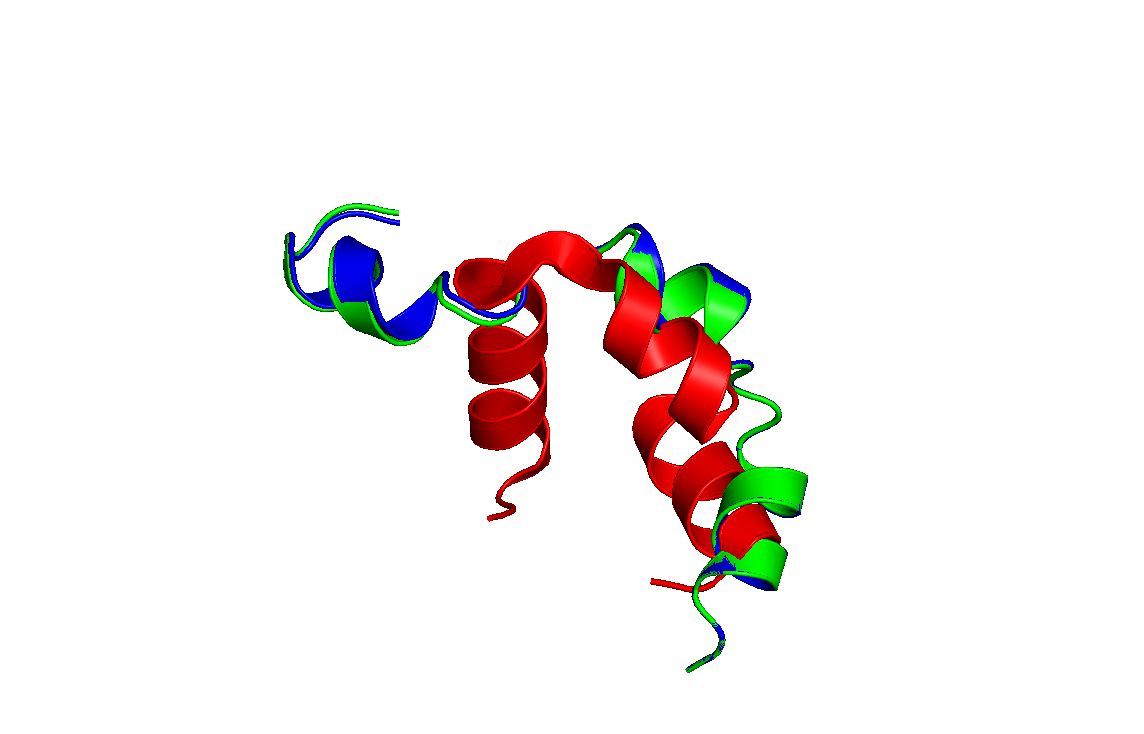
\includegraphics[width=8.5cm]{images/2F4K.png} & 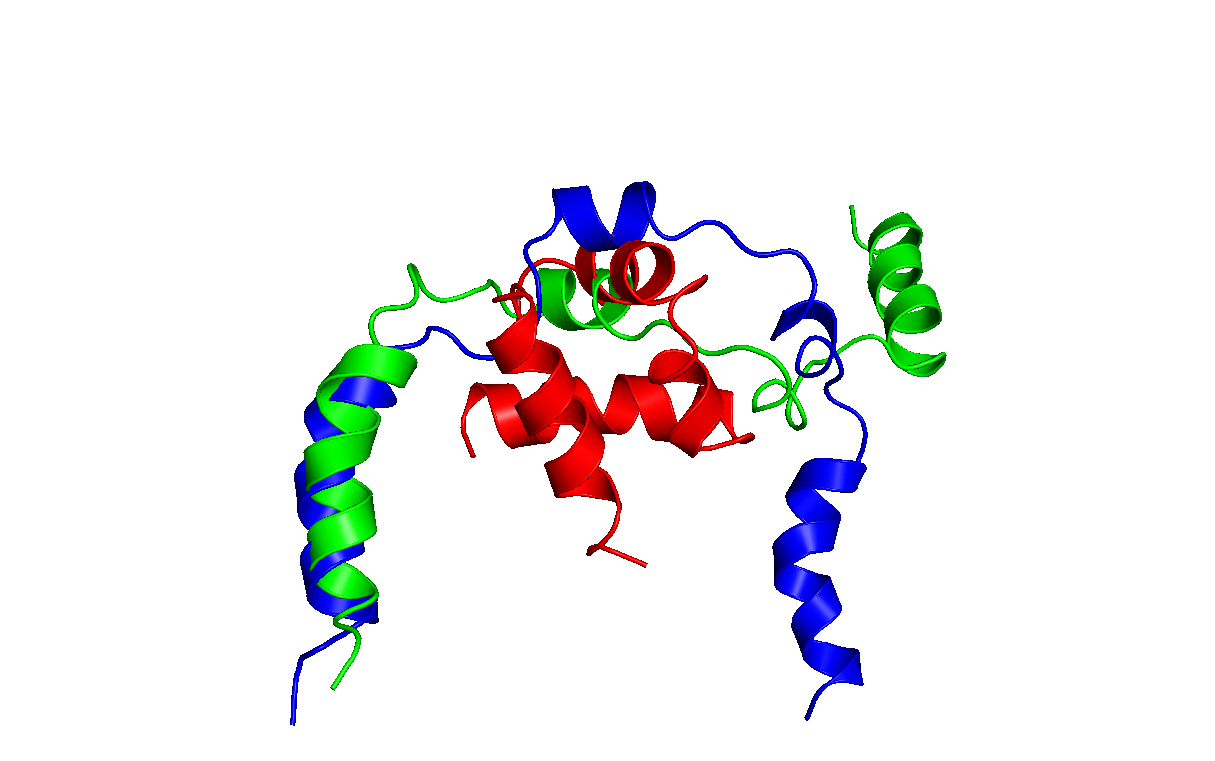
\includegraphics[width=8.5cm]{images/2JUC.png} \\
(a) & (b)\\
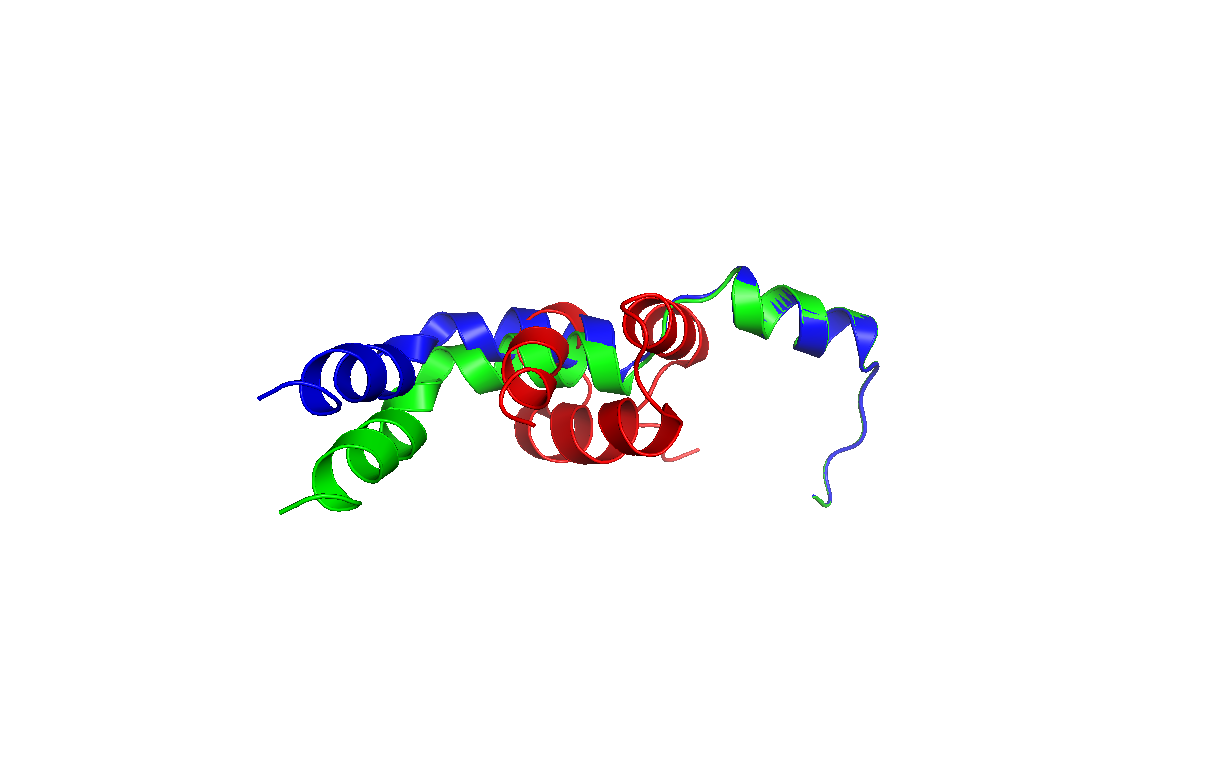
\includegraphics[width=8.5cm]{images/2MR9.png} & 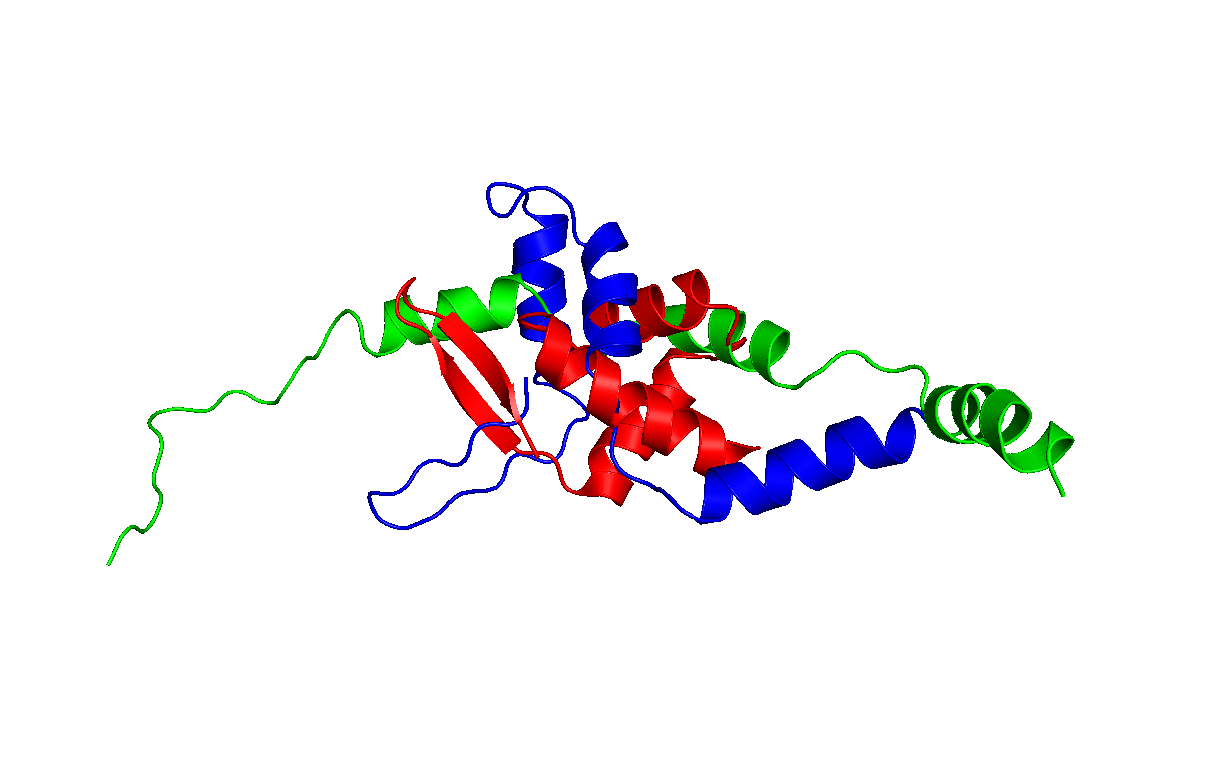
\includegraphics[width=8.5cm]{images/2P5K.png} \\
(c) & (d)\\
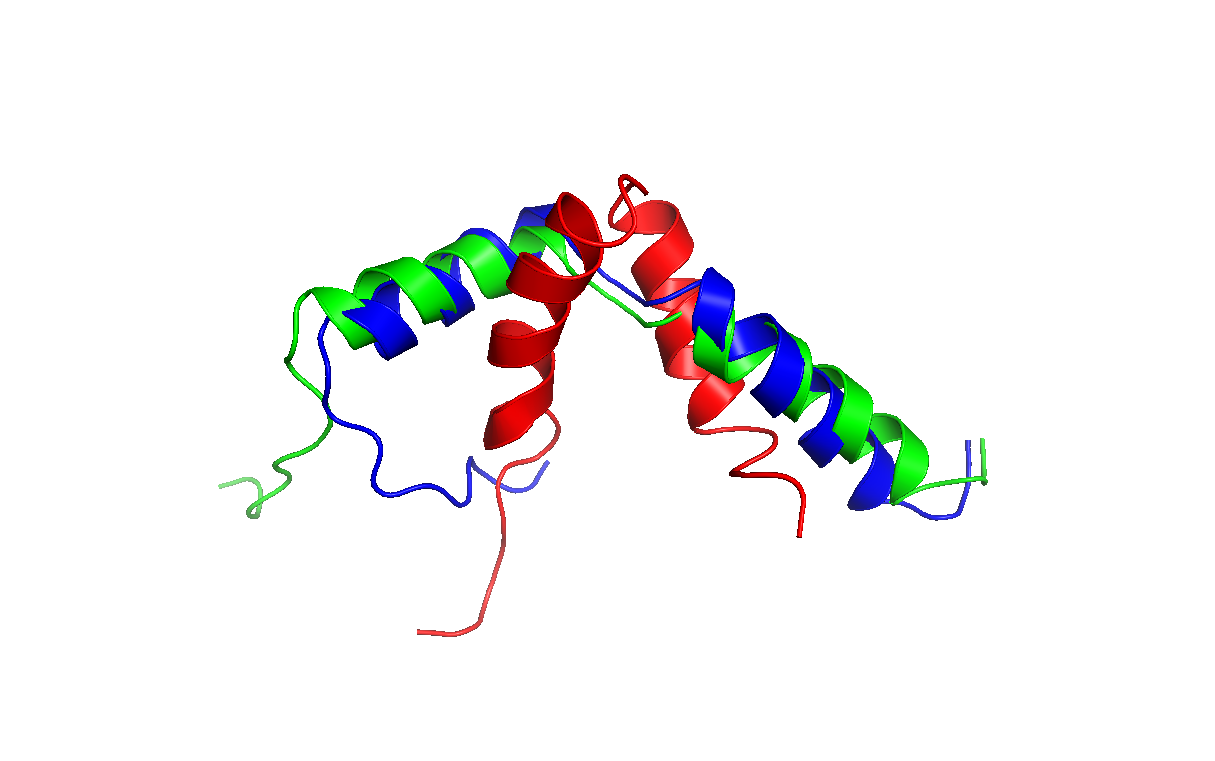
\includegraphics[width=8.5cm]{images/2P81.png} & 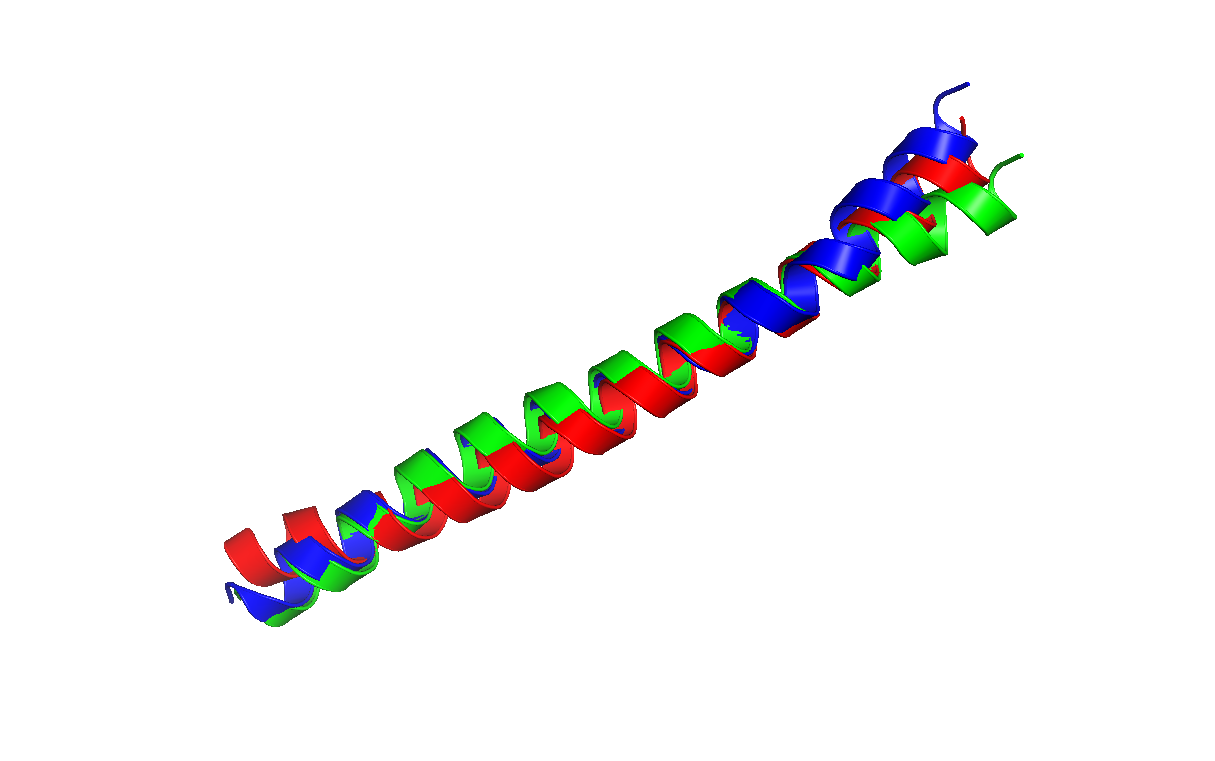
\includegraphics[width=8.5cm]{images/3P7K.png} \\
(e) & (f)\\
\end{tabular}
\caption[Alineación espacial de estructuras extensas]{Resultados de alineación espacial para las proteínas (a) 2F4K, (b) 2JUC, (c) 2MR9, (d) 2P5K, (e) 2P81 y (f) 3P7K. Solución con mejor energía en color verde, mejor RMSD en azul y estructura experimental en rojo. Las estructuras fueron alineadas a partir de la superposición de sus $C_{\alpha}$ utilizando PyMol.}
\label{fig:prot-ext-1}
\end{figure}

\begin{figure}
\centering
\begin{tabular}{c}
\\
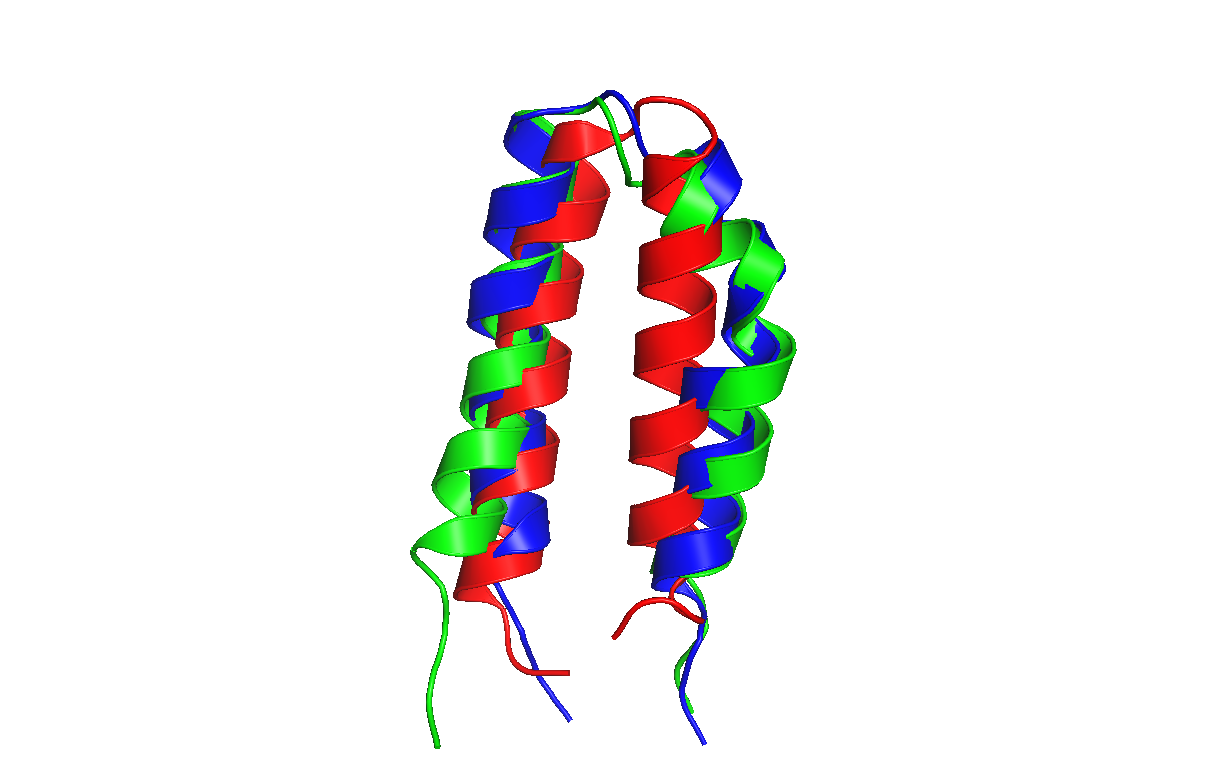
\includegraphics[width=8.5cm]{images/3V1A.png} \\
(g)\\
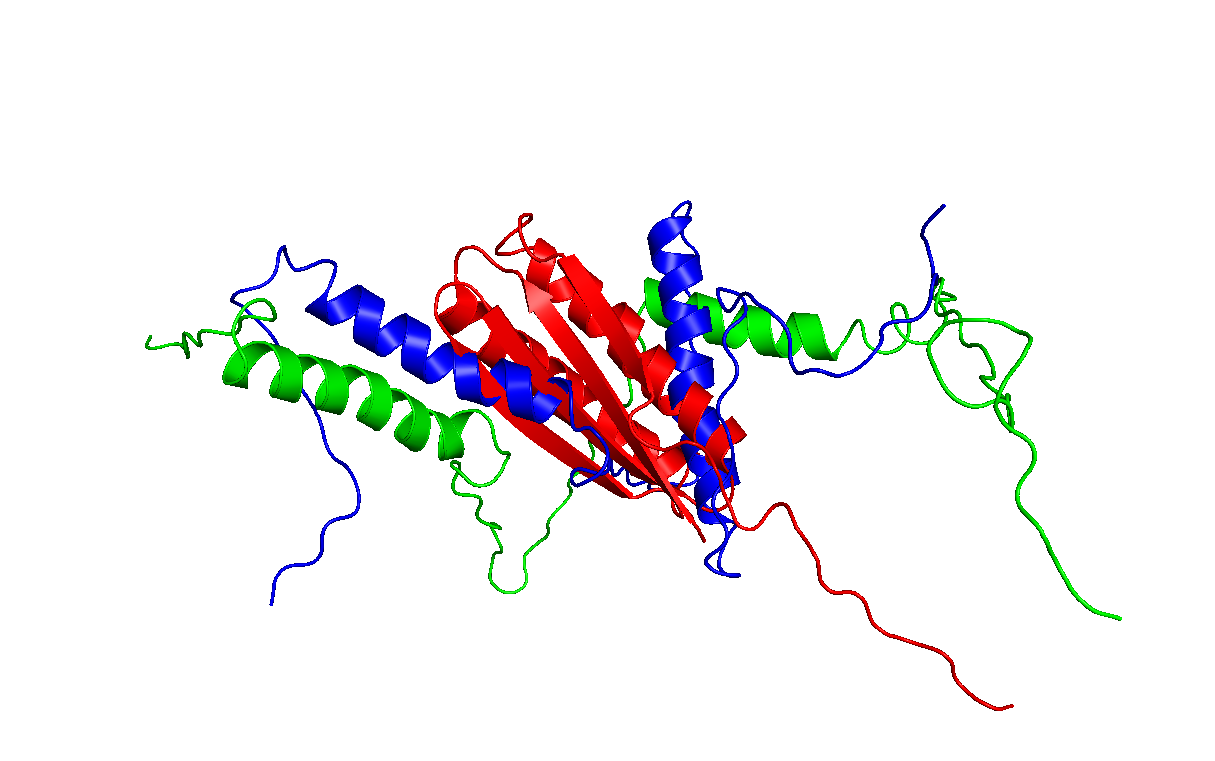
\includegraphics[width=8.5cm]{images/2MQ8.png} \\
(h)\\
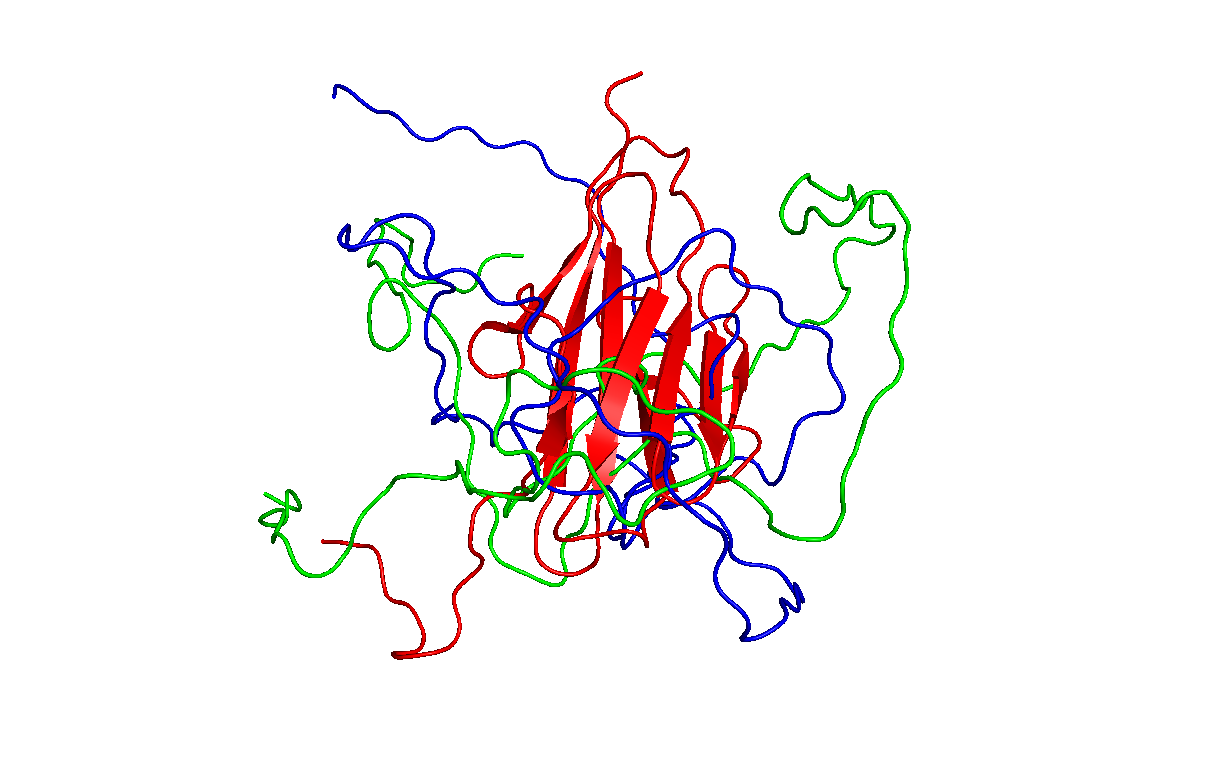
\includegraphics[width=8.5cm]{images/2MW1.png} \\
(i)\\
\end{tabular}
\caption[Alineación espacial de estructuras extensas]{Resultados de alineación espacial para las proteínas (g) 3V1A, (h) 2MQ8 e (i) 2MW1. Solución con mejor energía en color verde, mejor RMSD en azul y estrcutura experimental en rojo. Las estructuras fueron alineadas a partir de la superposición de sus $C_{\alpha}$ utilizando PyMol.}
\label{fig:prot-ext-2}
\end{figure}

Si bien, el MA a nivel de energía continúa encontrado buenas soluciones (energías bajas), sigue evidenciando el problema de predicción de las áreas de curvatura y hojas-$\beta$, no asi con las estructuras tipo hélices que se logran predecir de manera correcta.

Note que las proteínas 2MQ8 y 2MW1 son las más extensas y 72 horas fue tiempo insuficiente para su ejecución, debido a que no lograron llegar a las 50 generaciones. Queda expuesto de forma empírica que el incremento sustancial de aminoácidos en la secuencia implica un costo computacional elevado.

\chapter{Conclusiones}

En este trabajo se introdujo una nueva forma de solución para el problema \textit{3-D PSP}. La estrategia de solución implementa un algoritmo memético que incorpora, en el proceso de búsqueda, la información extraída de la \textit{Protein Data Bank (PDB)} en forma de Lista de Probabilidad de Ángulos (APL). Los resultados mostrados por el algoritmo propuesto muestran que puede encontrar buenas soluciones en términos de energía (valores negativos) y para algunos casos RMSD (menores a $2.6\AA$) cuando son comparadas con la estructura experimental. Adicionalmente, los resultados de los experimentos computacionales muestran la contribución positiva de las APLs al algoritmo, ya que conduce al MA y le permite obtener soluciones similares a las experimentales a nivel visual, no asi las que no usan APLs llegando a RMSDs de $>5\AA$. Esto se repite al evaluar el MA con proteínas extensas, si bien los resultados son bastante mayores que las proteínas en estudio, se debe recalcar que este problema es NP-Completo y el enfoque usado es de simulación \textit{ab initio}, lo que implica que cada vez que se evalúa una secuencia extensa implica un tiempo elevado, que repercute en la cantidad de generaciones, y en consecuencia, su convergencia a una solución.

Respecto a los problemas detectados a lo largo de la experimentación, se comprobó lo mencionado en \citealp{hornak:2006} sobre las falencias que presenta los campos de fuerza AMBER, resaltando la parametrización que presenta para la formación de hojas-$\beta$. Esto queda en evidencia al revisar que el MA no logra formar correctamente las hojas-$\beta$ y presenta problemas que repercuten en la conformación de las zonas en las que se producen peglamientos tipo \textit{Turn} o \textit{Coil}.

Sobre las herramientas para el desarrollo de \textit{software}, se debe mencionar la complejidad y nula flexibilidad del lenguaje de programación \textit{NAB} provisto por la \textit{suite AmberTools 14} para Modelamiento Molecular. Este problema causo en varias ocasiones cuellos de botella desde el punto de vista de la implementación. Además, esto presenta una desventaja para un plan de experimentación más amplio debido a que solo posee los campos de fuerza de \textit{Amber} y no permite probar otros como \textit{Charmm} o \textit{Rosetta}. Como solución, se podría usar el lenguaje Python con su bibliotecas para Modelamiento Molecular llamadas \textit{The Molecular Modelling Toolkit (MMTK)}, \textit{SIMTK} o \textit{PyOpenMM}.

Luego de la etapa de experimentación se desprenden interesantes aristas que podrían ser abarcadas en trabajos futuros. Medidas que pueden mejorar este trabajo parten por extender los histogramas que dan origen a las APLs usadas, se propone generar histogramas para residuos más específicos que consideren, además de la estructura secundaria, al residuo adyacente; lo que daría una cantidad de $8_{\text{e. secundaria}}{\times}20_{residuos}{\times}20_{residuos}=3200_{APL}$ y permitiría reducir aún más el espacio de búsqueda. Otra mejora que se plantea, es detectar aquellas zonas de la secuencia que se repiten a nivel de la población de agentes, para preservarlas y aplicar mayor esfuerzo computacional en aquellas zonas que son complejas de predecir. Como acotación final, cambiar el lenguaje de programación NAB permitiría usar los campos de fuerzas antes mencionados e incluso su combinación en el cálculo de energía, por ejemplo, podría usarse \textit{Rosseta} para las hojas-$\beta$ y \textit{Amber} para las hélices-$\alpha$ (ya que logra obtener RMSDs bajos menores a $2\AA$).

Finalmente, los resultados obtenidos fueron aceptados para su exposición en la \textit{Genetic and Evolutionary Computation Conference} (GECCO 2015) a efectuarse en Madrid, España los días 11 al 15 de Julio de 2015.
% ----------------------------------------------------------
% ----------- TERCERA PARTE --------------------------------
% \backmatter %Elimina la numeración
% ### Bibliografía de este documento ###
\bibliographystyle{apa-good}
\bibliography{referencias}
% ----------------------------------------------------------
% ----------- CUARTA PARTE ---------------------------------
%\appendix
%\addappheadtotoc %agregar Apéndice al índice. Si no tiene apéndices COMENTAR o BORRAR
% \noappendicestocpagenum %quitar número de páginas a los apéndices
% ### ANEXOS ###
%%--------Apendice

 % Manuales de Usuario
\end{document}
%\\end
